\documentclass{beamer}

%%% -------------- CREATE HANDOUTS -----------------------------------
%\documentclass[12pt, handout]{beamer}
%\usepackage{pgfpages}
%\pgfpagesuselayout{4 on 1}[letterpaper, landscape, border shrink=5mm]
%%% ------------------------------------------------------------------


\mode<presentation>
  \usepackage{ru}
  %\usetheme{Warsaw}
  %\usecolortheme{seahorse}
  %\usefonttheme{default}
  \setbeamertemplate{caption}[numbered]
  \setbeamertemplate{headline}{}
  %\setbeamertemplate{navigation symbols}{}
  \setbeamertemplate{bibliography item}[text]
\newcommand*\oldmacro{}%
	\let\oldmacro\insertshorttitle%
%\renewcommand*\insertshorttitle{%
%   \oldmacro\hfill%
%   \insertframenumber\,/\,\inserttotalframenumber}
\setbeamertemplate{section page}{
    \begin{centering}
    \vspace{1cm}
    \begin{beamercolorbox}[rounded=true,shadow=false,sep=4pt,center]{part title}
    \usebeamerfont{section title}\LARGE{\insertsection}\par
    \end{beamercolorbox}
    \end{centering}}
\usepackage{ragged2e}
\usepackage[english]{babel}
\usepackage[utf8]{inputenc}
\usepackage{appendixnumberbeamer}
\usepackage{natbib}
\usepackage{textpos}
\usepackage{lipsum}
\usepackage{tikz}
\usepackage[percent]{overpic}
\usepackage{textcomp}
\usepackage{booktabs}
\usepackage{mathabx}
\usepackage{pifont}
\usepackage{bbding}
\usepackage{fontenc}
%\let\Sun\undefined   %to undefine something
%\usepackage{marvosym}
%\usepackage{scalerel}
%% \usepackage[
%%   style=numeric,
%%   citestyle=authoryeartitle
%% ]{biblatex}
\setbeamerfont{caption}{size=\tiny}

%\usepackage[usenames,dvipsnames]{color}
\usepackage{listings}
\usepackage{courier} % Required for the courier font
\usepackage{mathtools}


% define ``struts'', as suggested by Claudio Beccari in
%    a piece in TeX and TUG News, Vol. 2, 1993.
\newcommand\Tstrut{\rule{0pt}{2.6ex}}         % = `top' strut
\newcommand\Bstrut{\rule[-0.9ex]{0pt}{0pt}}   % = `bottom' strut

%--------------------------------------------------------------------
%	CODE INCLUSION CONFIGURATION
%---------------------------------------------------------------------
% This is the color used for comments
\definecolor{MyDarkGreen}{rgb}{0.0,0.4,0.0}
\definecolor{Blue}{rgb}{0.0,0.0,0.5}
\lstloadlanguages{Perl,Python} % Load Perl syntax for listings,
% for a list of other languages supported see:
%ftp://ftp.tex.ac.uk/tex-archive/macros/latex/contrib/listings/listings.pdf
\lstset{language=Perl, % Use Perl in this example
        frame=single, % Single frame around code
        basicstyle=\tiny\ttfamily, % Use small true type font
        %keywordstyle=[1]\color{Blue}\bf, % Perl functions bold and blue
        %keywordstyle=[2]\color{Purple}, % Perl function arguments purple
        % Custom functions underlined and blue
        %keywordstyle=[3]\color{Blue}\underbar, 
        identifierstyle=, % Nothing special about identifiers
        % Comments small dark green courier font
        %commentstyle=\usefont{T1}{pcr}{m}{sl}\color{MyDarkGreen}\small, 
        %stringstyle=\color{Purple}, % Strings are purple
        showstringspaces=false, % Don't put marks in string spaces
        tabsize=5, % 5 spaces per tab
        %
        % Put standard Perl functions not included
        % in the default language here
        morekeywords={rand},
        %
        % Put Perl function parameters here
        morekeywords=[2]{on, off, interp},
        %
        % Put user defined functions here
        morekeywords=[3]{test},
       	%
        % Line continuation (...) like blue comment
        %morecomment=[l][\color{Blue}]{...}, 
        numbers=left, % Line numbers on left
        firstnumber=1, % Line numbers start with line 1
        numberstyle=\tiny\color{White}, % Line numbers are blue and small
        %numberstyle=\tiny
        stepnumber=5 % Line numbers go in steps of 5
}

\lstset{language=Python, % Use Python in this example
        frame=single, % Single frame around code
        basicstyle=\small\ttfamily, % Use small true type font
        keywordstyle=[1]\color{Blue}\bf, % Python functions bold and blue
        keywordstyle=[2]\color{Purple}, % Python function arguments purple
        % Custom functions underlined and blue
        keywordstyle=[3]\color{Blue}\underbar, 
        identifierstyle=, % Nothing special about identifiers
        % Comments small dark green courier font
        commentstyle=\usefont{T1}{pcr}{m}{sl}\color{MyDarkGreen}\small, 
        stringstyle=\color{Purple}, % Strings are purple
        showstringspaces=false, % Don't put marks in string spaces
        tabsize=3, % 5 spaces per tab
        %
        % Put standard Python functions not included in the
        % default language here
        morekeywords={rand},
        %
        % Put Python function parameters here
        morekeywords=[2]{on, off, interp},
        %
        % Put user defined functions here
        morekeywords=[3]{test},
       	%
        % Line continuation (...) like blue comment
        morecomment=[l][\color{Blue}]{...}, 
        numbers=left, % Line numbers on left
        firstnumber=1, % Line numbers start with line 1
        numberstyle=\tiny\color{Blue}, % Line numbers are blue and small
        stepnumber=5 % Line numbers go in steps of 5
}

% Creates a new command to include a perl script, the first
% parameter is the filename of the script (without .inp), the
% second parameter is the caption
\newcommand{\inputdeck}[2]{
\begin{itemize}
\item[]\lstinputlisting[caption=#2,label=#1,language=Perl]{#1.inp}
\end{itemize}
}

\newcommand{\inputdeckpages}[3]{
\begin{itemize}
\item[]\lstinputlisting[label=#1,language=Perl,
       firstline=#2,lastline=#3,basicstyle=\scriptsize]{#1.inp}
\end{itemize}
}

%\lstinputlisting[language=Octave, firstline=2, lastline=12]{BitXorMatrix.m}

\newcommand{\pythonscript}[2]{
\begin{itemize}
\item[]\lstinputlisting[caption=#2,label=#1]{#1}
\end{itemize}
}

\newcommand{\pythonscriptpages}[3]{
  \begin{itemize}
  \item[]\lstinputlisting[label=#1,language=Python,
    firstline=#2,lastline=#3,basicstyle=\scriptsize]{#1.inp}
  \end{itemize}
}

%\setbeameroption{show notes}
%\setbeamertemplate{note page}[plain]
\newcommand{\tss}{\textsuperscript}
\newcommand{\tsbs}{\textsubscript}
%Change Bullets in latex list
\setbeamertemplate{itemize item}{\scriptsize\raise1.25pt\hbox{\donotcoloroutermaths\ding{118}}}
\setbeamertemplate{itemize subitem}{\scriptsize\raise1.25pt\hbox{\ding{226}}}
\setbeamertemplate{itemize subsubitem}{\tiny\raise1.25pt\hbox{\ding{169}}}
\setbeamertemplate{enumerate item}{\insertenumlabel.}

\usepackage{pifont}
\newcommand{\cmark}{\ding{51}}%
\newcommand{\xmark}{\ding{55}}%
\newcommand{\done}{\rlap{$\square$}{\raisebox{2pt}{\large\hspace{1pt}\cmark}}%
  \hspace{-2.5pt}}
\newcommand{\wontfix}{\rlap{$\square$}{\large\hspace{1pt}\xmark}}
\newcommand{\ndone}{\rlap{$\square$}{\raisebox{2pt}{}}%
  \hspace{8pt}}

%%To select specific font
%{\fontsize{2.5}{4}\selectfont tobesize}

%\setbeamertemplate{background}{\tikz[overlay, remember picture]\node[xshift=-2.3cm, yshift=1.50cm, opacity=0.4]at (current page.south east){
\includegraphics[width=4cm]{images}};}

\title[Depletion Calculation UQ]{Uncertainty quantification of depletion calculations for specific isotopes using ORIGEN2}
\author{Paul Mendoza}
\date{December 6, 2016}

\begin{document}
\setbeamertemplate{caption}{\raggedright\insertcaption\par}
\begin{frame}
	%% background
  \tikz[overlay, remember picture]\node[xshift=-3.5cm, yshift=3cm, opacity=0.1]at (current page.south east){
\includegraphics[width=8cm]{tamu_system_proposed_seal_042915}};
	%% Left-hand logo
  %% \begin{tikzpicture}[remember picture, overlay]
  %% \node [xshift = 3 cm, yshift=1.2cm] at (current page.south west){
\includegraphics[width=5cm]{tees_logo_primary_maroon}};
  %% \end{tikzpicture}
    %% Right-hand logo
  \begin{tikzpicture}[remember picture, overlay]
  \node [xshift = -3cm, yshift=1.2cm] at (current page.south east){
\includegraphics[width=5cm]{TEES_NSSPI_logo_HMaroon}};
  \end{tikzpicture}
  %% Upper logo right
    \begin{tikzpicture}[remember picture,overlay]
    \node[anchor=north east,yshift=2pt] at (current page.north east) {
\includegraphics[height=0.8cm]{NUENlogo}};
    \end{tikzpicture}
  %% Upper logo left
    %% \begin{tikzpicture}[remember picture,overlay]
    %% \node[anchor=north west,yshift=2pt] at (current page.north west) {
\includegraphics[height=0.8cm]{NUENlogo}};
    %% \end{tikzpicture}
    \titlepage
    \vspace{-1.8cm}
    \begin{center}
      Presented for NUEN647
    \end{center}
\end{frame}

%Add Biola Seal
\setbeamertemplate{background}{\tikz[overlay, remember picture]\node[xshift=-2.5cm, yshift=2.5cm, opacity=0.05]at (current page.south east){
\includegraphics[width=6cm]{imageedit_2_7317234434}};}

%% %Add NSSPI to upper right
%% \addtobeamertemplate{frametitle}{}{%
%%   \begin{tikzpicture}[remember picture,overlay]
%%     \node[anchor=north east,yshift=2pt] at (current page.north east) {
\includegraphics[height=0.8cm]{TEES_NSSPI_Acronym_logo_WHT}};
%%     \end{tikzpicture}}



\begin{frame}{Outline}
\tableofcontents
\end{frame}

\section{Background}
\subsection{Introduction}
\begin{frame}{Introduction}
  %\vspace{-1cm}
  \begin{itemize}
  \item{Determing composition of irradiated fuel importance}
    \begin{itemize}
    \item{Flux calculations}
    \item{Reprocessing}
    \item{Irradiation history verification}
    \end{itemize}
  \item{Usually determined with a type of Bateman solver}
  \item{Uncertainties rarely reported}
    \begin{itemize}
    \item{Flux Shape}
    \item{Fission yield}
    \item{\textbf{Cross Sections}}
    \item{Half-lives}
    \end{itemize}
  \end{itemize}
\end{frame}

\subsection{Current Problem}
\begin{frame}{Current Problem}
  \begin{columns}
    \begin{column}{0.6\textwidth}
      %\vspace{10mm}
      \begin{itemize}
      \item{Use of depletion code ORIGEN2}
        \begin{itemize}
        \item{Solves with exponential method}
        \item{Requires libraries}
          \begin{itemize}
          \item{Decay information}
          \item{Fission yield data}
          \item{Single group cross sections}
          \end{itemize}
        \end{itemize}
      \item{PWR system with 3 wt\% enriched uranium}
      \item{Varied $\sigma_\gamma$
        and $\sigma_f$ for: \tss{235}U, \tss{238}U,
        \tss{239}Pu, \tss{240}Pu, and \tss{241}Pu}
        \begin{itemize}
        \item{Originally, $\sigma_\gamma$ and $\gamma$ for
          the FP were considered}
        \end{itemize}
      \end{itemize}
    \end{column}
    \begin{column}{0.4\textwidth}
      \begin{table}[H]
        \begin{center}
          \caption{\large{Quantities of Interest}}
          \label{Table:1}
          \begin{tabular}{l l l}
            \toprule
            \tss{133}Cs & \tss{136}Ba & \tss{153}Eu\\
            \tss{134}Cs & \tss{138}Ba & \tss{154}Eu\\
            \tss{135}Cs & \tss{149}Sm & \tss{239}Pu\\
            \tss{137}Cs & \tss{150}Sm & \tss{242}Pu\\
            \tss{148}Nd & \tss{106}Rh & \tss{125}Sb\\
            \bottomrule
          \end{tabular}
        \end{center}
      \end{table}
    \end{column}
  \end{columns}  
\end{frame}


\section{Objectives}
\begin{frame}
  \begin{block}{Objectives}
  \vspace{0.3cm}
  \begin{itemize}
  \item[\ndone]{Build ORIGEN2 model for thermal system, calculating
  concentrations of QOIs}
  \item[\ndone]{Determine how to vary cross section inputs for calculation}
  \item[\ndone]{Determine variance of cross-sections}
  \item[\ndone]{Create a sampling space for all possible variations of
    calculations}
  \item[\ndone]{Write program to plot results}
  \end{itemize}
  \vspace{0.3cm}
\end{block}
\end{frame}



\subsection{ORIGEN2 Model}
\begin{frame}{ORIGEN2 Model}
  \begin{itemize}
  \item{Model irradiates 1 metric ton of US PWR fuel for a single
    cycle (15,000 MWd/Mt)}
  \item{Constant power assumption (37.5 W/g)}
  \item{Does not include oxygen}
  \item{Verified with \tss{137}Cs content}
  \end{itemize}
  \vspace{4mm}
  \begin{center}
    \small
    $
    \frac{552.8\ \text{g \tss{137}Cs}}{Mt}\cdot
    \frac{6.022E23\ \text{atoms}}{137\ \text{g \tss{137}Cs}}\cdot
    \frac{\text{Fission}}{0.06\ \text{atoms}}\cdot
    \frac{200\ \text{MeV}}{\text{Fission}}\cdot
    \frac{1.602E-19\ \text{MJ}}{1\ \text{MeV}}\cdot
    \frac{1\ \text{day}}{86400\ \text{s}}=15,018\ \frac{\text{MWd}}{Mt}$
  \end{center}
\end{frame}

\begin{frame}{ORIGEN2 Model}
  \inputdeckpages{../Origen2/TAPE5}{4}{25} %11
\end{frame}


\begin{frame}
  \begin{block}{Objectives}
    \vspace{0.3cm}
  \begin{itemize}
  \item[\done]{Build ORIGEN2 model for thermal system, calculating
  concentrations of QOIs}
  \item[\ndone]{Determine how to vary cross section inputs for calculation}
  \item[\ndone]{Determine variance of cross-sections}
  \item[\ndone]{Create a sampling space for all possible variations of
    calculations}
  \item[\ndone]{Write program to plot results}
  \end{itemize}
  \vspace{0.3cm}
\end{block}
\end{frame}


\subsection{Cross Section Variations}
\begin{frame}{How the manual says it is\tss{\tiny{\AsteriskThin}}...}
  \vspace{5mm}
  \begin{itemize}
  \item{TAPE9.inp (8th input on LIB card)}
  \item{TAPE8.inp (9th input on LIB card)}
    \begin{itemize}
    \item{Sorry for the confusion}
    \end{itemize}
  \item{LPU card}
    \begin{itemize}
    \item{Short for Lost Plutonium\tss{\tiny{\AsteriskThin}}}
    \end{itemize}
  \item{Programed both, neither worked}
    \begin{itemize}
    \item{The first lied to my face}
    \item{The second complained about:
      ``An endfile record was detected in a READ statement (unit= 8)''}
    \item{Didn't find out about the lying until last night}
    \end{itemize}
  \end{itemize}

  \begin{table}[H]
  \begin{center}
    \label{Table:2}
    \resizebox{\textwidth}{!}{%
    \begin{tabular}{l l l l l l l l l}
      \toprule
      LIB & NUCLID & (n,$\gamma$) & (n,2n) & (n,3n) &
      (n,f) & (n,$\gamma^*$) & (n,2n\tss{*}) & YYN\\
      %LIB & Y(\tss{232}Th) & Y(\tss{233}U) & Y(\tss{235}U) &
      %Y(\tss{238}U) & Y(\tss{239}Pu) & Y(\tss{241}Pu) &
      %Y(\tss{245}Cm) & Y(\tss{249}Cf)\\
      \bottomrule
    \end{tabular}}
  \end{center}
  \end{table}

  \vspace{1.3cm}
  \textsuperscript{\tiny{\AsteriskThin\hspace{1mm} Its not Really}}  
\end{frame}


\begin{frame}
  \begin{block}{Objectives}
    \vspace{0.3cm}
  \begin{itemize}
  \item[\done]{Build ORIGEN2 model for thermal system, calculating
  concentrations of QOIs}
  \item[\wontfix]{Determine how to vary cross section inputs for calculation}
  \item[\ndone]{Determine variance of cross-sections}
  \item[\ndone]{Create a sampling space for all possible variations of
    calculations}
  \item[\ndone]{Write program to plot results}
  \end{itemize}
  \vspace{0.3cm}
\end{block}
\end{frame}



\subsection{Variance for cross-sections}
\begin{frame}{Cross-section calculations}

  \begin{equation*}
    \sigma=\frac{\int\sigma(E)\phi(E)dE}{\int\phi(E)dE}
  \end{equation*}

  \begin{align*}
    \phi(E) =& C_1\cdot \frac{E}{E_0^2} \cdot
    exp\left(-\frac{E}{E_0}\right) &&E<E_{max,th}\\
    =& \frac{C_2}{E}  &&E_{max,th}<E<E_{max,epi}\\
    =& C_3 \cdot \frac{\sqrt{\frac{E}{E_f}}}{E_f}
    \cdot exp\left(-\frac{E}{E_{f}}
    \right) &&E>E_{max,epi}
  \end{align*}


  {\tiny
    \setlength{\abovedisplayskip}{6pt}
    \setlength{\belowdisplayskip}{\abovedisplayskip}
    \setlength{\abovedisplayshortskip}{0pt}
    \setlength{\belowdisplayshortskip}{3pt}
    \begin{align*}
      C_1=&\frac{E_0^2}{E^2_{max,th}}e^{E_{max,th}/E_0}
      \\
      C_2=&1\\
      C_3=&\frac{E_f}{E_{max,epi}}
      \cdot
      e^{\frac{E_{max,epi}}{E_f}}\frac{1}
      {\sqrt{\frac{E_{max,epi}}{E_f}}}
    \end{align*}
    }%
  {\tiny
  $E_{max,th}=0.50\ \text{eV}$,
  $E_{max,epi}=1E5\ \text{eV}$,
  $\theta_{th}=0.09\ \text{eV}$ (764 K),
  $\theta_{fis}=1.35E6\ \text{eV}$}%
\end{frame}

\begin{frame}{Difference Minimization}
  \begin{figure}[H]
    \begin{center}
      \hspace*{-0.9cm}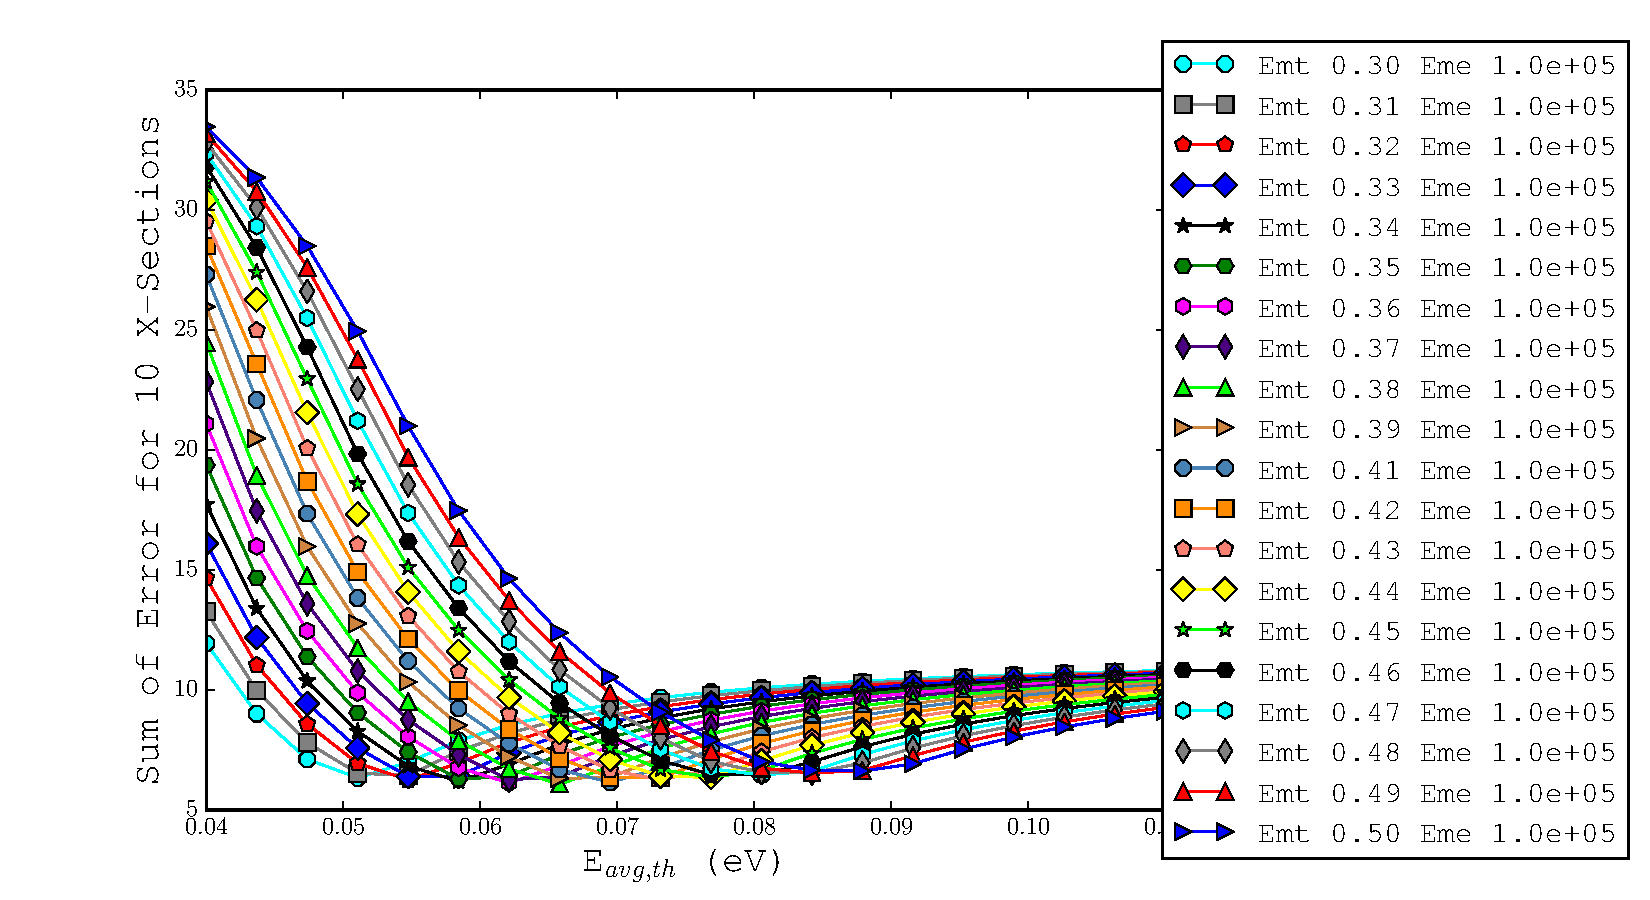
\includegraphics[width=1.1\columnwidth]{../Weighting/Reduce_Err/E0_vs_SumErr_third.pdf}
      \vspace{-5mm}
      \label{fig:err}
    \end{center}
  \end{figure}
\end{frame}

\begin{frame}{Flux Distribution}
  \begin{figure}[H]
    \begin{center}
      \hspace*{-0.5cm}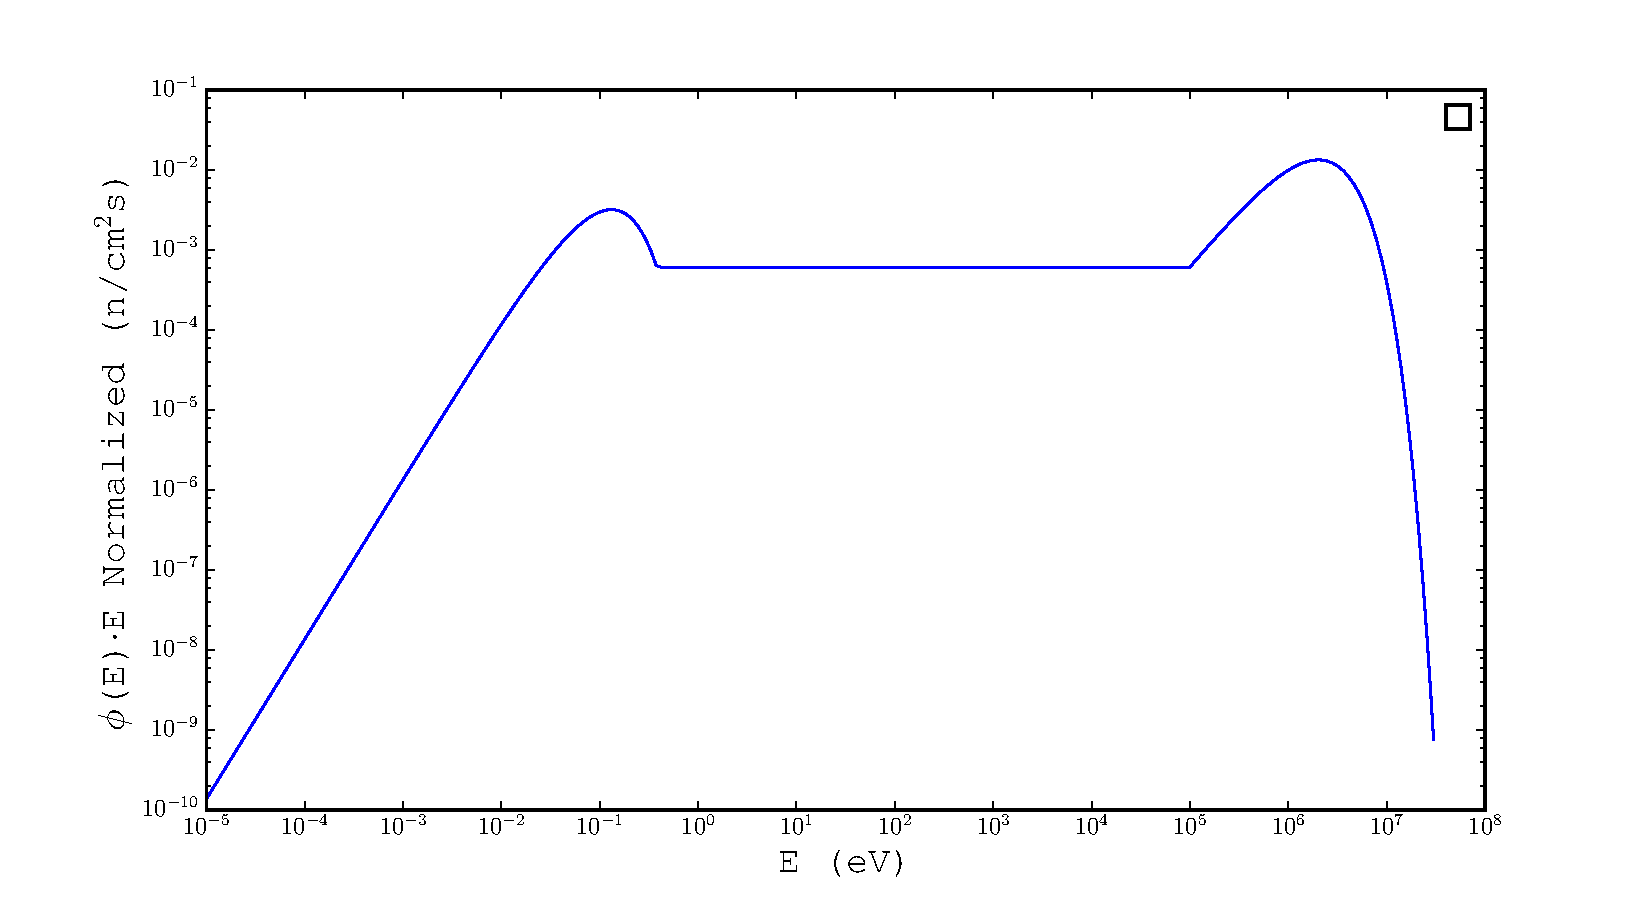
\includegraphics[width=1.1\columnwidth]{../Weighting/Flux_Spectra.pdf}
      \vspace{-5mm}
      \label{fig:Flux}
    \end{center}
  \end{figure}
\end{frame}

\begin{frame}{One Group Cross Section Comparison}
  \vspace{-4mm}
  \begin{table}[H]
  \begin{center}
    \resizebox{\textwidth}{!}{%
    \begin{tabular}{l l l l}
      \toprule
      Isotope\tss{Rxn} & ENDF VII & ORIGEN2 & Ratio\Tstrut\Bstrut\\
      \hline
      \tss{239}Pu\tss{$\gamma$} & 6.544e+01 & 6.909E+01 & 1.06\Tstrut\\
      \tss{240}Pu\tss{$\gamma$} & 1.521e+02 & 2.228E+02 & 1.46\\
      \tss{241}Pu\tss{$\gamma$} & 4.518e+01 & 4.202E+01 & 0.93\\
      \tss{235}U\tss{$\gamma$}  & 9.387e+00 & 1.068E+01 & 1.14\\
      \tss{238}U\tss{$\gamma$}  & 4.098e+00 & 8.872E-01 & 0.22\\
      \tss{239}Pu\tss{f} & 1.179e+02 & 1.211E+02 & 1.03\\
      \tss{240}Pu\tss{f} & 9.609e-01 & 5.787E-01 & 0.60\\
      \tss{241}Pu\tss{f} & 1.253e+02 & 1.259E+02 & 1.01\\
      \tss{235}U\tss{f}  & 4.621e+01 & 4.752E+01 & 1.03\\
      \tss{238}U\tss{f}  & 2.091e-01 & 9.281E-02 & 0.44\\
      \bottomrule
    \end{tabular}}
  \end{center}
  \end{table}
\end{frame}

\begin{frame}
  \begin{figure}[H]
    \begin{center}
      \hspace*{-0.7cm}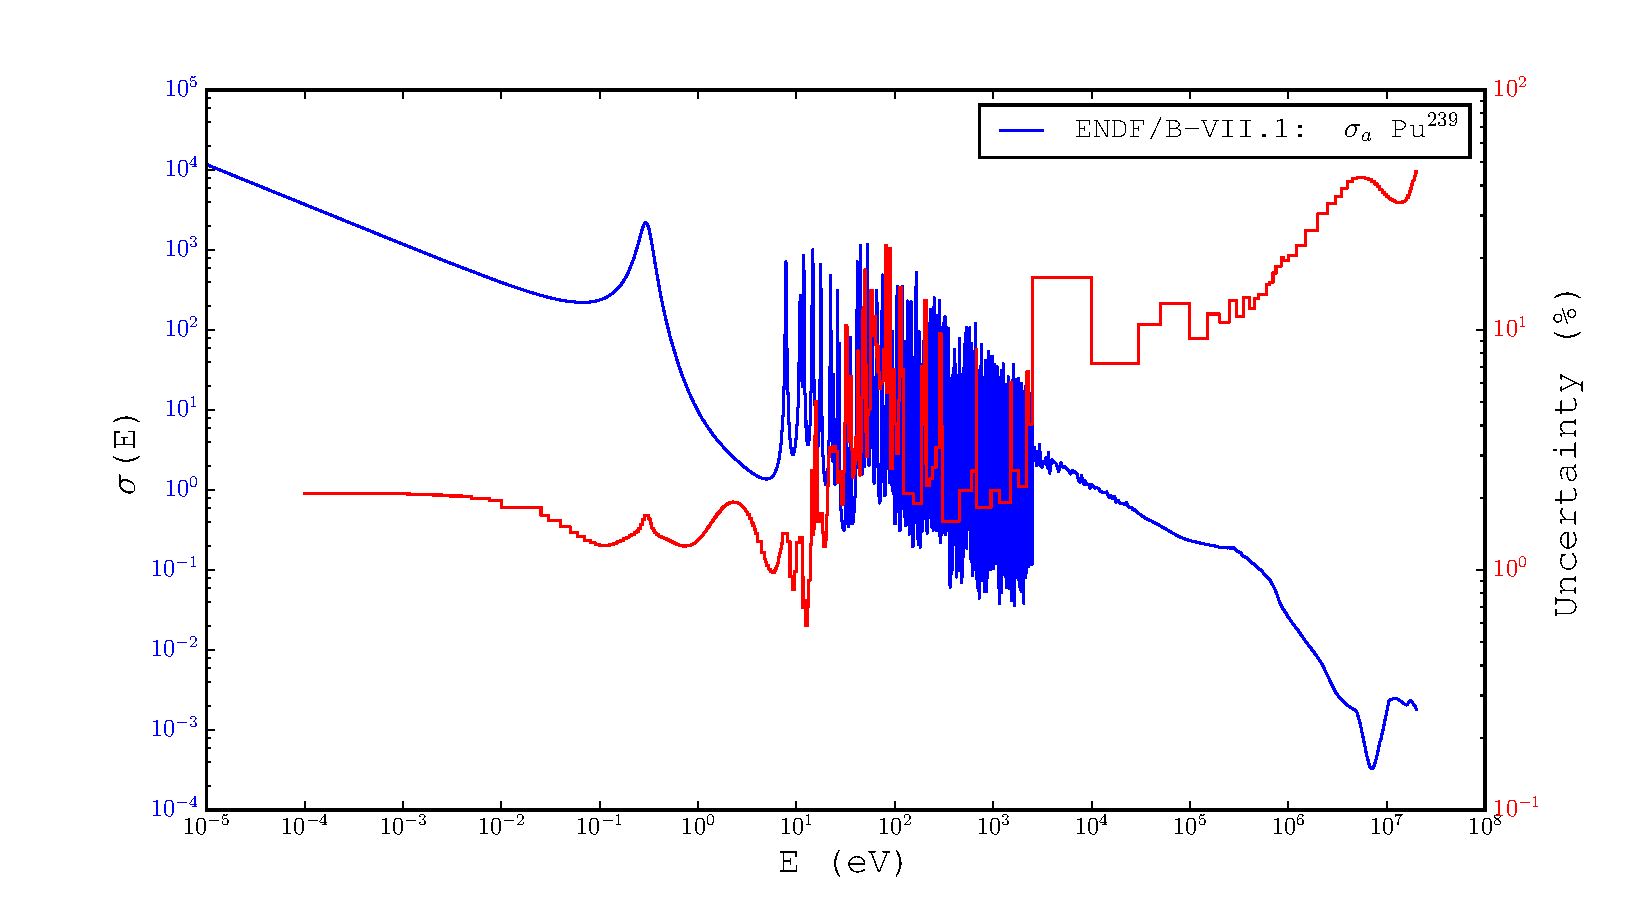
\includegraphics[width=1.1\columnwidth]{../Weighting/X_Sections/XwVar_Pu_239_94_a.pdf}
      \vspace{-5mm}
      \label{fig:XPu239}
    \end{center}
  \end{figure}
\end{frame}

\begin{frame}
    \begin{figure}[H]
    \begin{center}
      \hspace*{-0.7cm}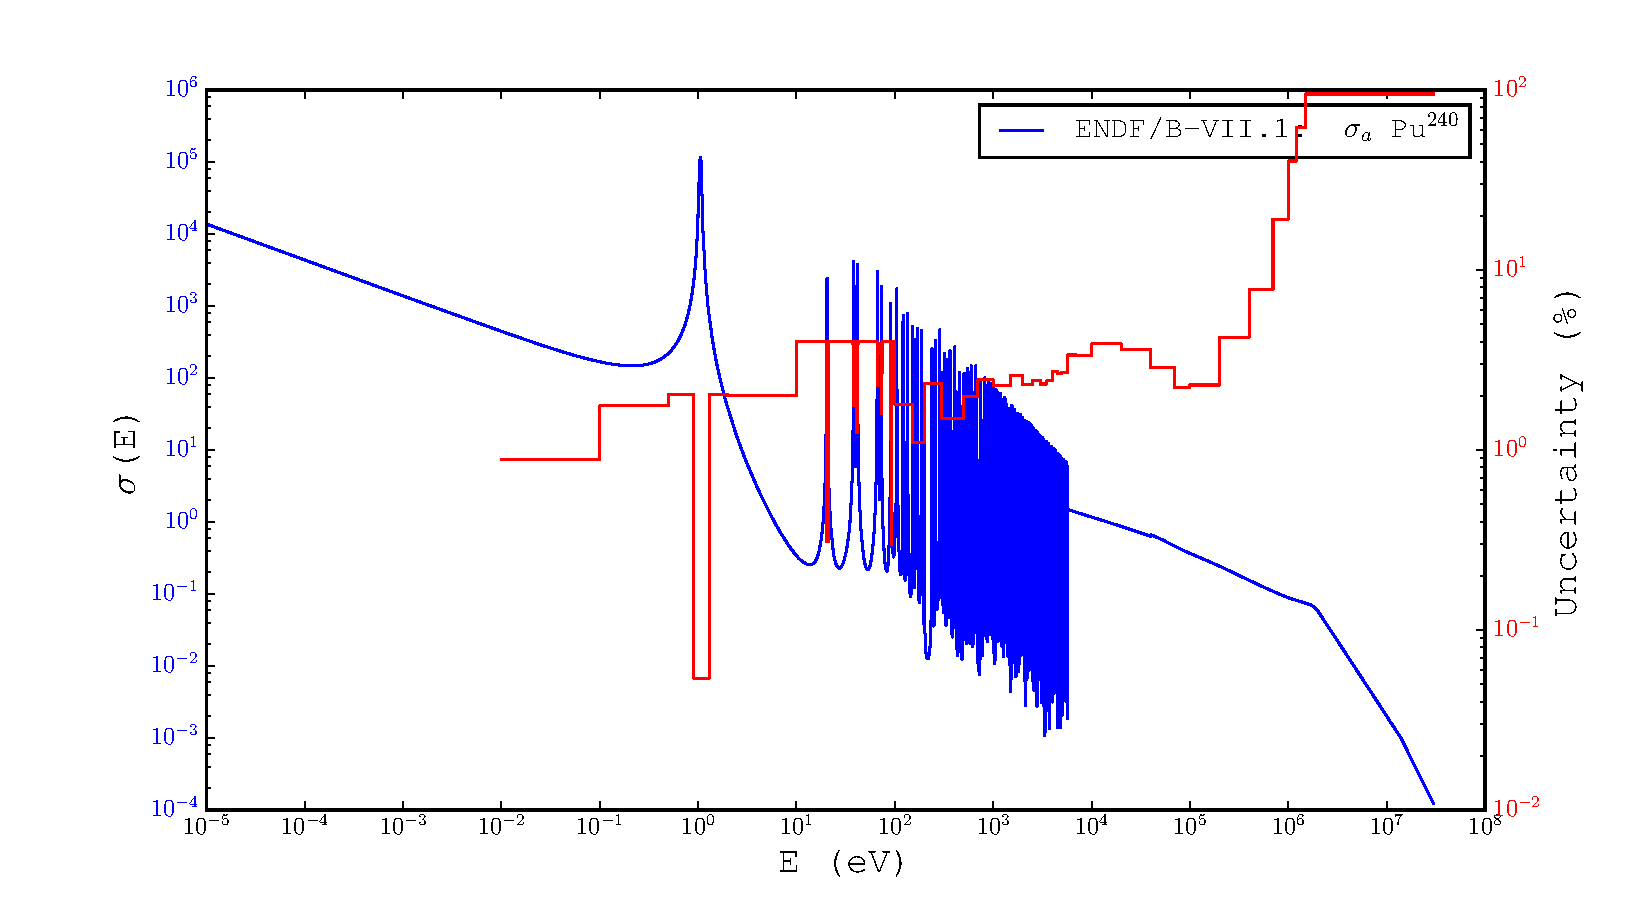
\includegraphics[width=1.1\columnwidth]{../Weighting/X_Sections/XwVar_Pu_240_94_a.pdf}
      \vspace{-5mm}
      \label{fig:XPu240}
    \end{center}
  \end{figure}
\end{frame}

\begin{frame}
    \begin{figure}[H]
    \begin{center}
      \hspace*{-0.7cm}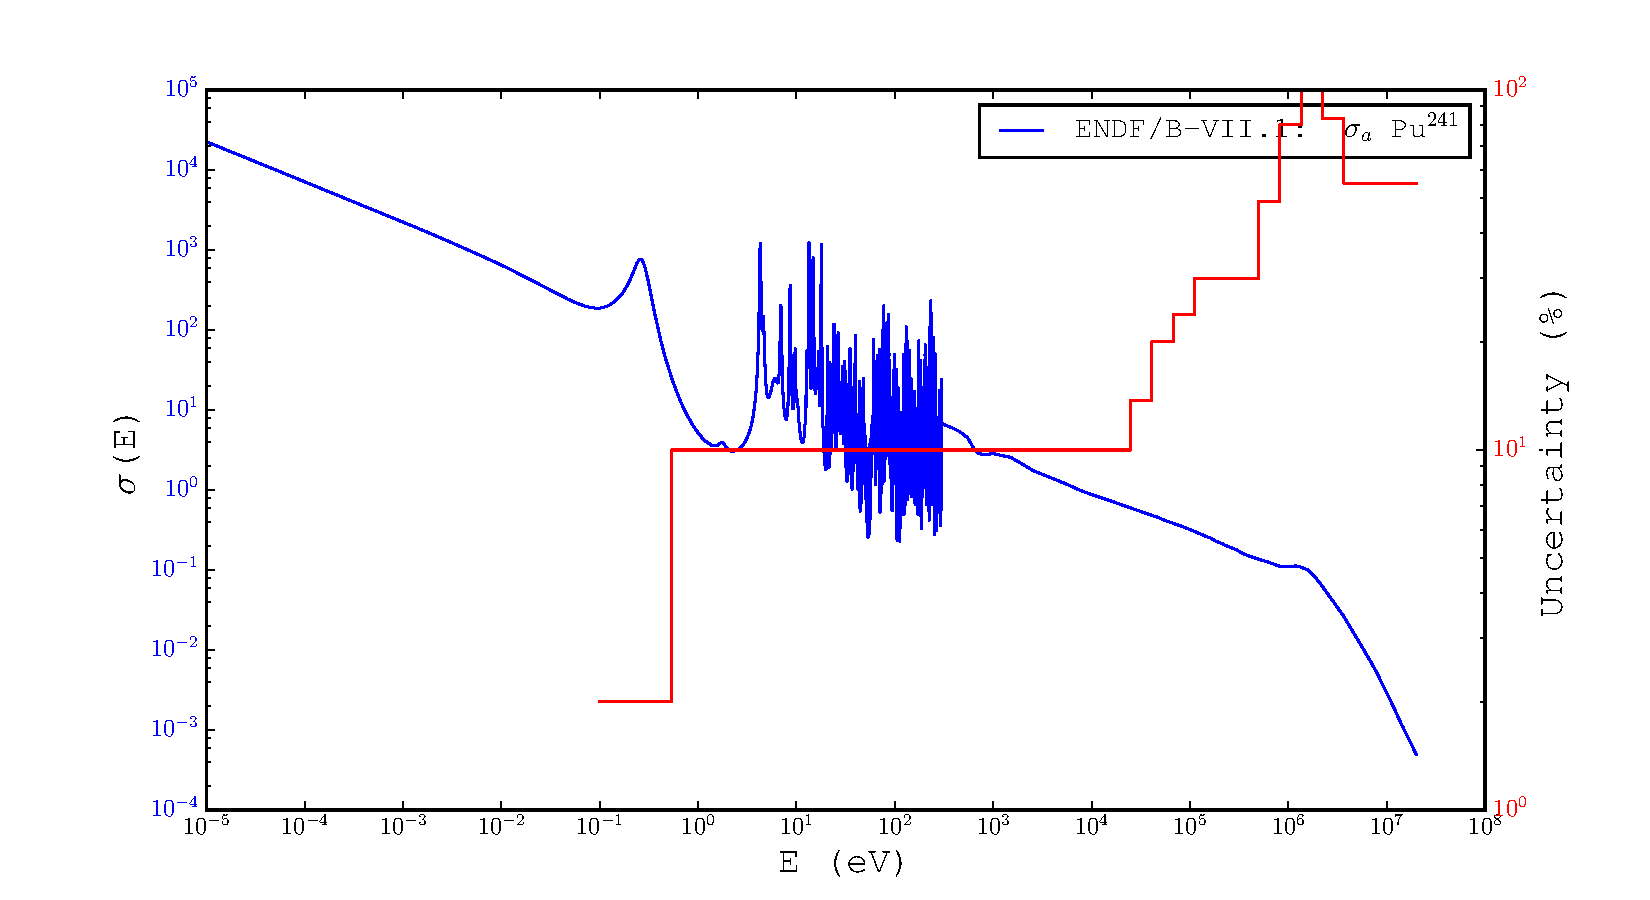
\includegraphics[width=1.1\columnwidth]{../Weighting/X_Sections/XwVar_Pu_241_94_a.pdf}
      \vspace{-5mm}
      \label{fig:XPu241}
    \end{center}
  \end{figure}
\end{frame}

\begin{frame}
  \begin{figure}[H]
    \begin{center}
      \hspace*{-0.7cm}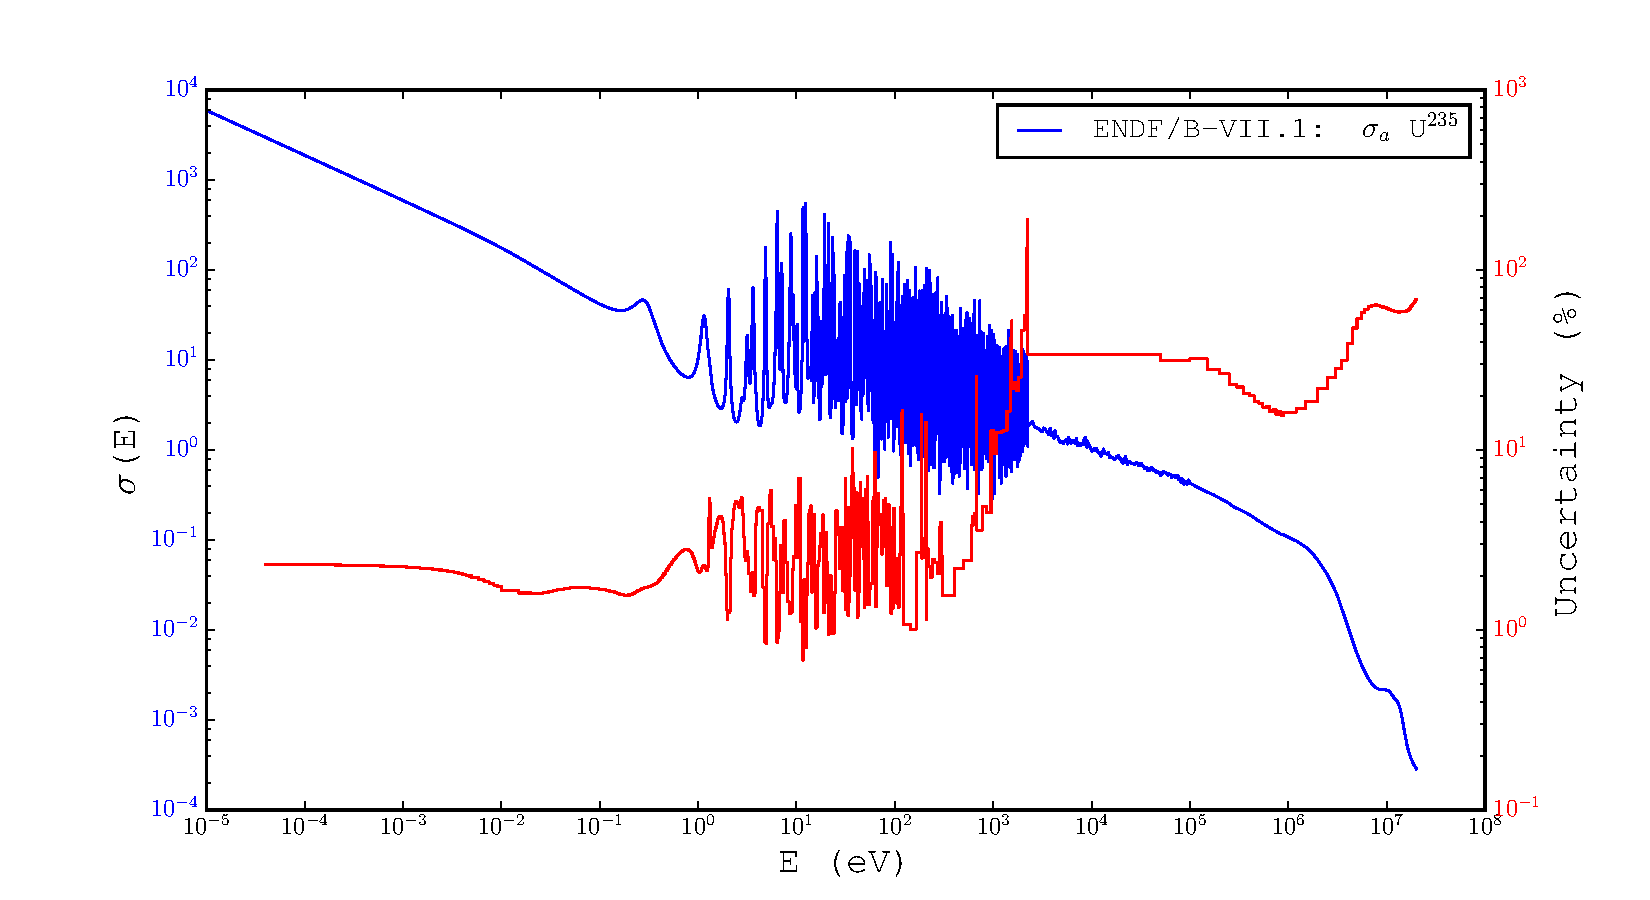
\includegraphics[width=1.1\columnwidth]{../Weighting/X_Sections/XwVar_U_235_92_a.pdf}
      \vspace{-5mm}
      \label{fig:XU235}
    \end{center}
  \end{figure}
\end{frame}

\begin{frame}
  \begin{figure}[H]
    \begin{center}
      \hspace*{-0.7cm}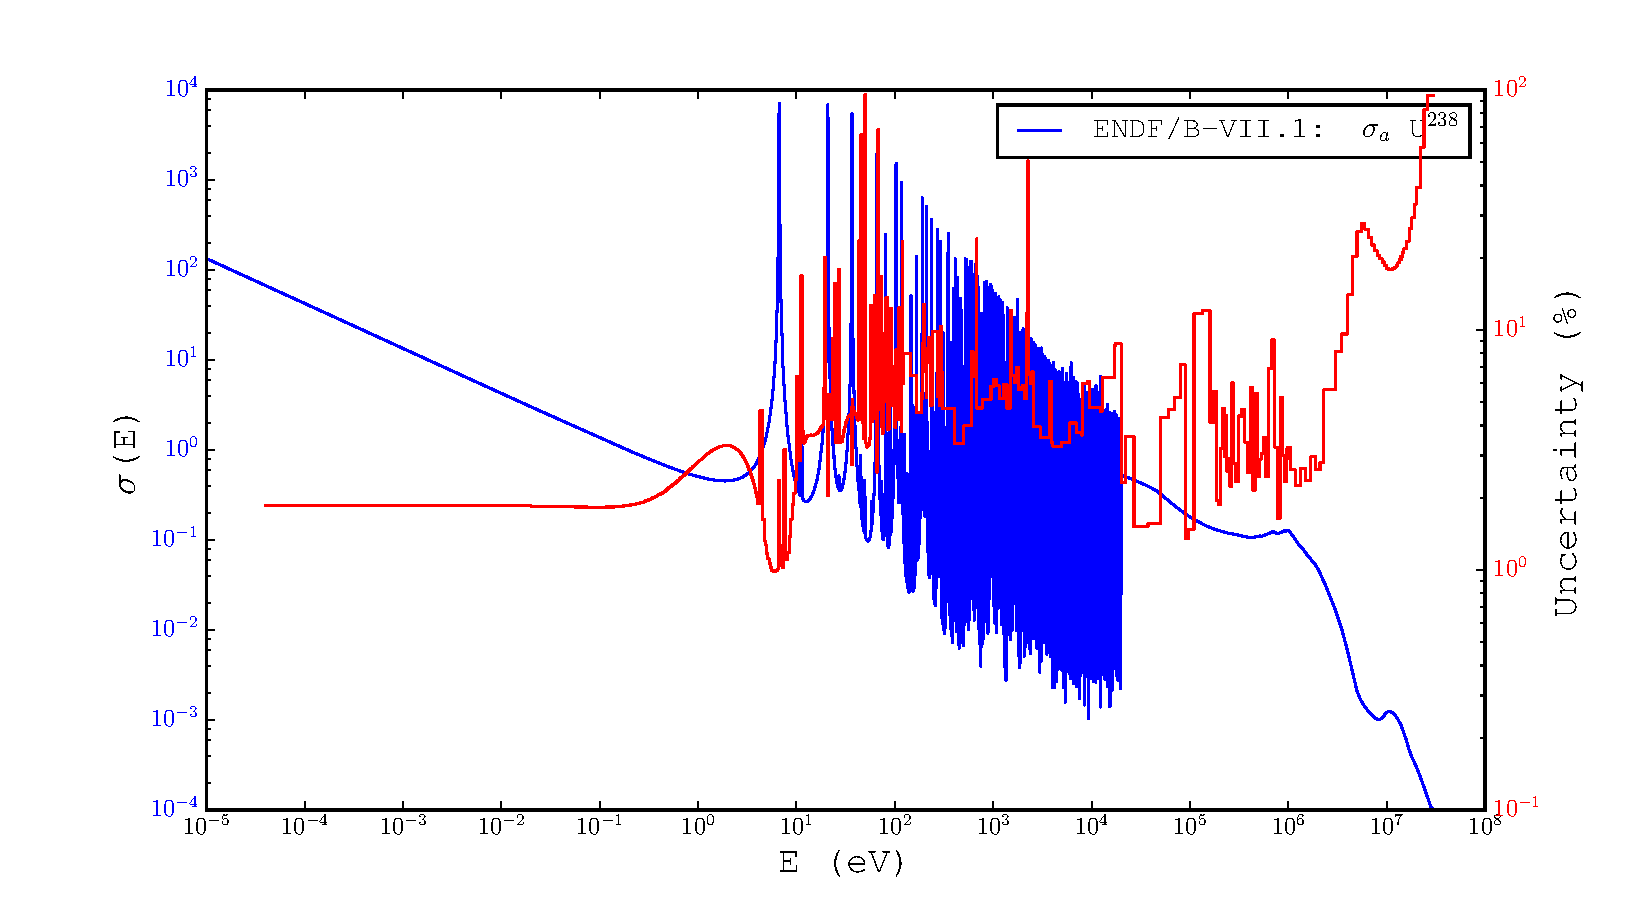
\includegraphics[width=1.1\columnwidth]{../Weighting/X_Sections/XwVar_U_238_92_a.pdf}
      \vspace{-5mm}
      \label{fig:XU238}
    \end{center}
  \end{figure}
\end{frame}

\begin{frame}
  \begin{figure}[H]
    \begin{center}
      \hspace*{-0.7cm}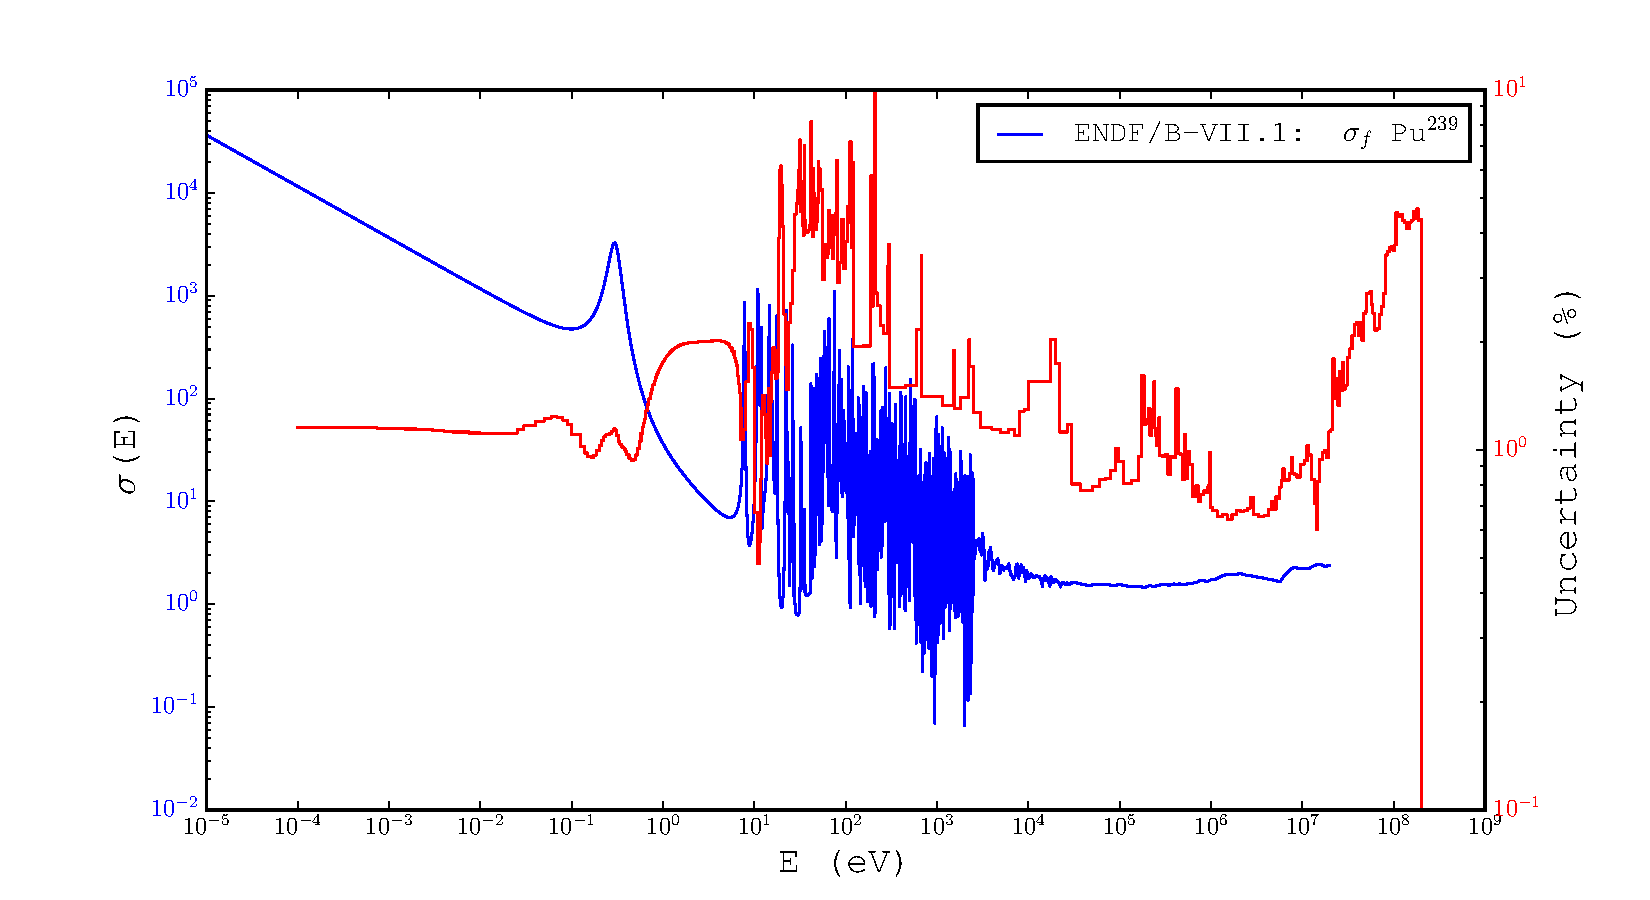
\includegraphics[width=1.1\columnwidth]{../Weighting/X_Sections/XwVar_Pu_239_94_f.pdf}
      \vspace{-5mm}
      \label{fig:XPu239}
    \end{center}
  \end{figure}
\end{frame}

\begin{frame}
    \begin{figure}[H]
    \begin{center}
      \hspace*{-0.7cm}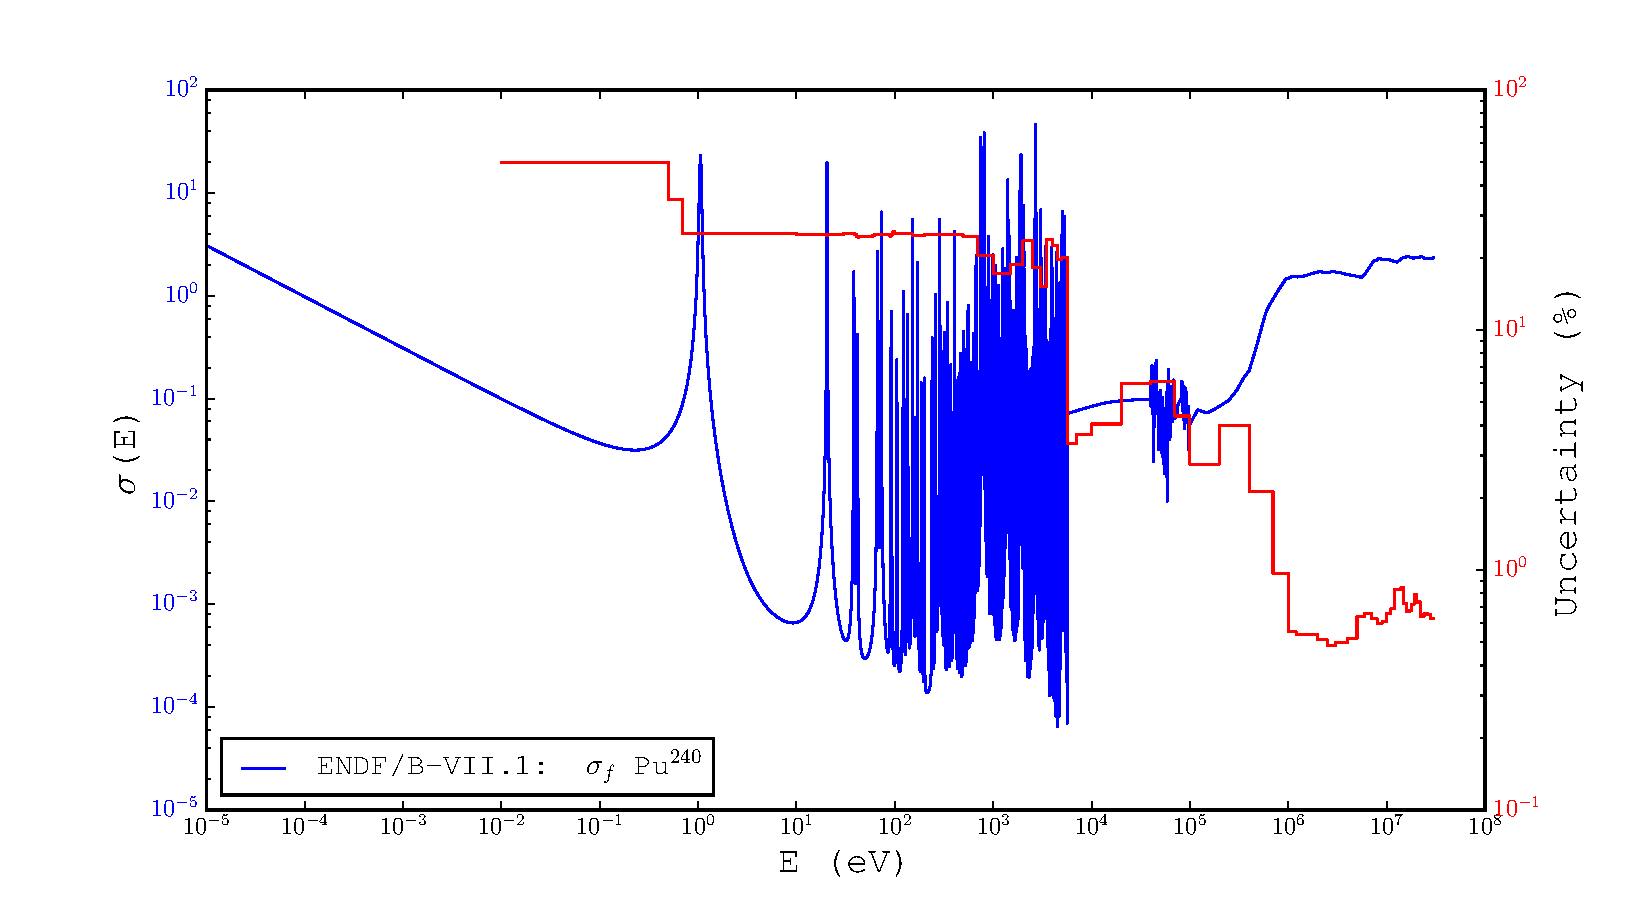
\includegraphics[width=1.1\columnwidth]{../Weighting/X_Sections/XwVar_Pu_240_94_f.pdf}
      \vspace{-5mm}
      \label{fig:XPu240}
    \end{center}
  \end{figure}
\end{frame}

\begin{frame}
    \begin{figure}[H]
    \begin{center}
      \hspace*{-0.7cm}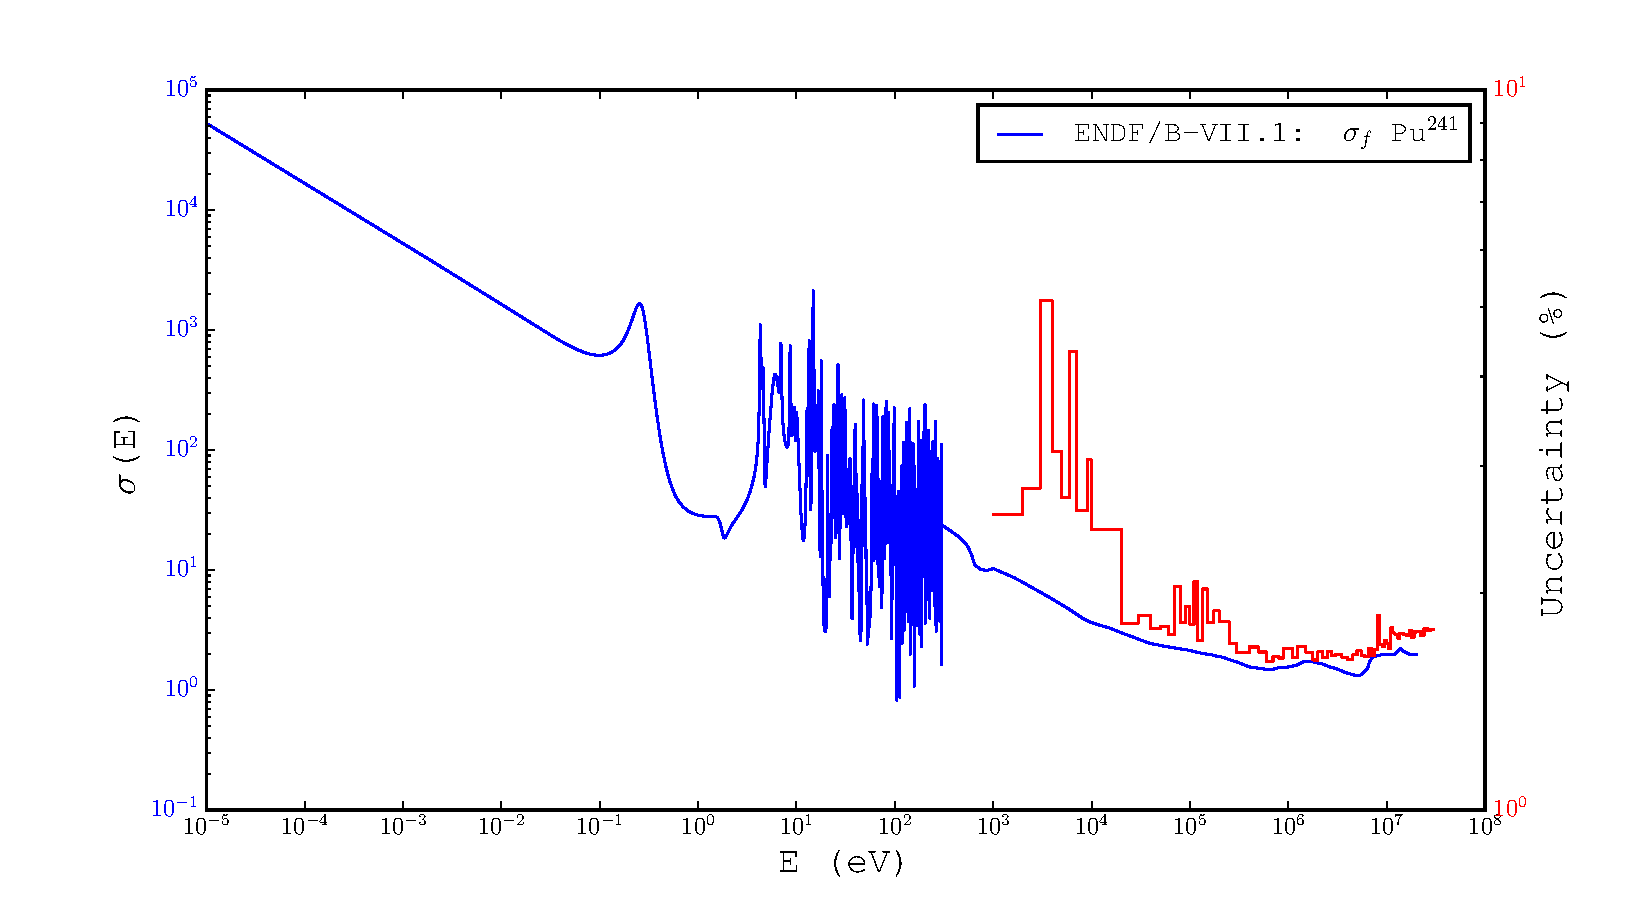
\includegraphics[width=1.1\columnwidth]{../Weighting/X_Sections/XwVar_Pu_241_94_f.pdf}
      \vspace{-5mm}
      \label{fig:XPu241}
    \end{center}
  \end{figure}
\end{frame}

\begin{frame}
  \begin{figure}[H]
    \begin{center}
      \hspace*{-0.7cm}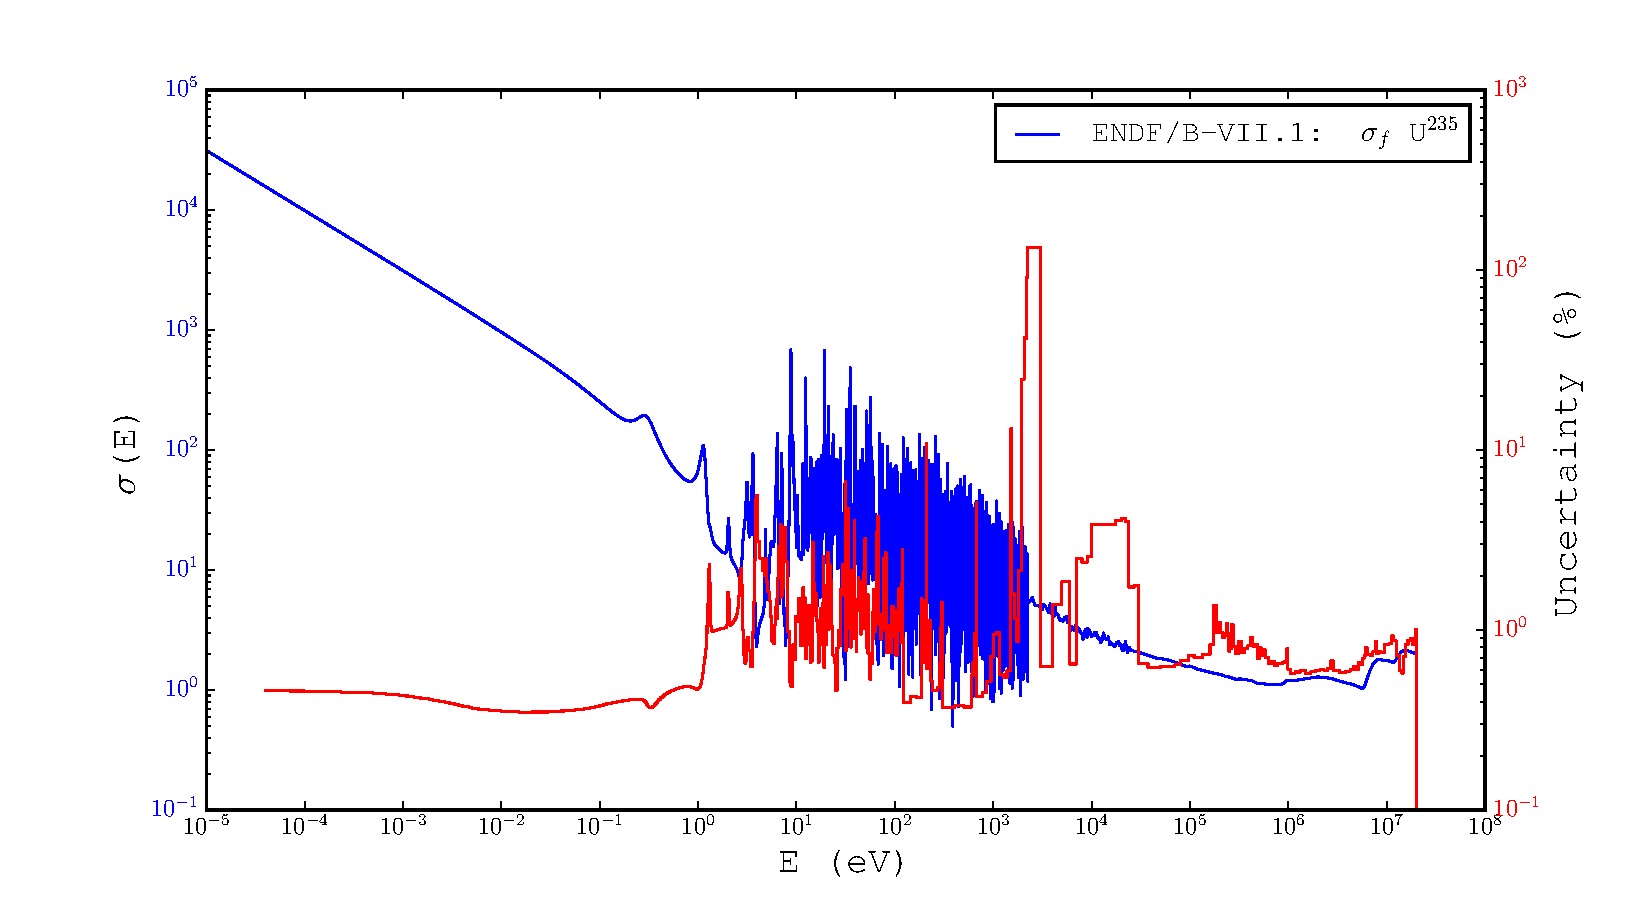
\includegraphics[width=1.1\columnwidth]{../Weighting/X_Sections/XwVar_U_235_92_f.pdf}
      \vspace{-5mm}
      \label{fig:XU235}
    \end{center}
  \end{figure}
\end{frame}

\begin{frame}
  \begin{figure}[H]
    \begin{center}
      \hspace*{-0.7cm}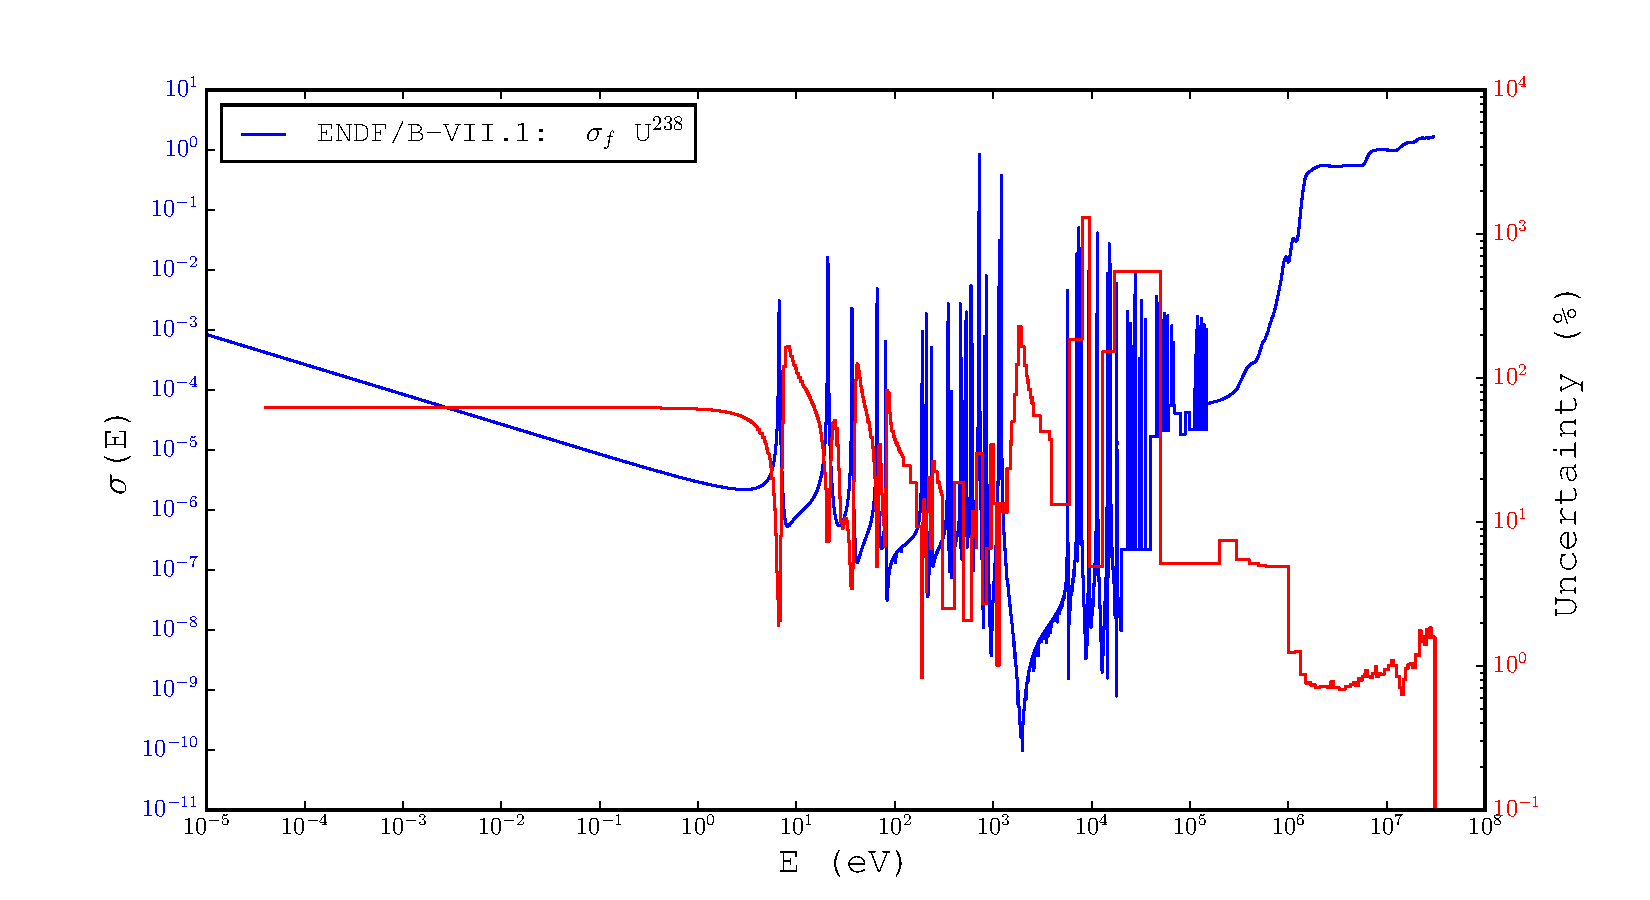
\includegraphics[width=1.1\columnwidth]{../Weighting/X_Sections/XwVar_U_238_92_f.pdf}
      \vspace{-5mm}
      \label{fig:XU238}
    \end{center}
  \end{figure}
\end{frame}

\begin{frame}{Single Group Cross Sections with Errors}
  \begin{table}[H]
  \begin{center}
    \label{Table:4}
    \begin{tabular}{l l}
      \toprule
      Isotope\tss{Rxn} & $\sigma$ with 1STD Error\Tstrut\Bstrut\\
      \hline
      \tss{239}Pu\tss{$\gamma$} & 69.09$\pm$8.15\Tstrut\\
      \tss{240}Pu\tss{$\gamma$} & 222.8$\pm$50.9\\
      \tss{241}Pu\tss{$\gamma$} & 42.02$\pm$10.92\\
      \tss{235}U\tss{$\gamma$}  & 10.68$\pm$3.23\\
      \tss{238}U\tss{$\gamma$}  & 0.887$\pm$0.175\\
      \tss{239}Pu\tss{f} & 121.1$\pm$1.2 \\
      \tss{240}Pu\tss{f} & 0.579$\pm$0.003 \\
      \tss{241}Pu\tss{f} & 125.9$\pm$2.3 \\
      \tss{235}U\tss{f}  & 47.52$\pm$0.71 \\
      \tss{238}U\tss{f}  & 0.093$\pm$8.2e-7 \\
      \bottomrule
    \end{tabular}
  \end{center}
  \end{table}
\end{frame}

\begin{frame}
  \begin{block}{Objectives}
  \vspace{0.3cm}
  \begin{itemize}
  \item[\done]{Build ORIGEN2 model for thermal system, calculating
  concentrations of QOIs}
  \item[\wontfix]{Determine how to vary cross section inputs for calculation}
  \item[\done]{Determine variance of cross-sections}
  \item[\ndone]{Create a sampling space for all possible variations of
    calculations}
  \item[\ndone]{Write program to plot results}
  \end{itemize}
  \vspace{0.3cm}
\end{block}
\end{frame}


\subsection{Sampling Space and Plotting Program}
\begin{frame}{Sampling space and Plotting}
  \begin{equation*}
    \pi(\theta)=\frac{\theta^{\alpha-1}e^{-\theta/\beta}}{\Gamma(\alpha)
      \beta^{\alpha}},\ \ \ \ \ \theta,\alpha,\beta>0.
  \end{equation*}
  \vspace{1cm}
  \begin{equation*}
    \alpha=\frac{\text{Mean}^2}{\text{Error}^2}
  \end{equation*}
  \begin{equation*}
    \beta=\frac{\text{Error}^2}{\text{Mean}}
  \end{equation*}
\end{frame}


\begin{frame}
  \begin{figure}[H]
    \begin{center}
      \hspace*{-0.6cm}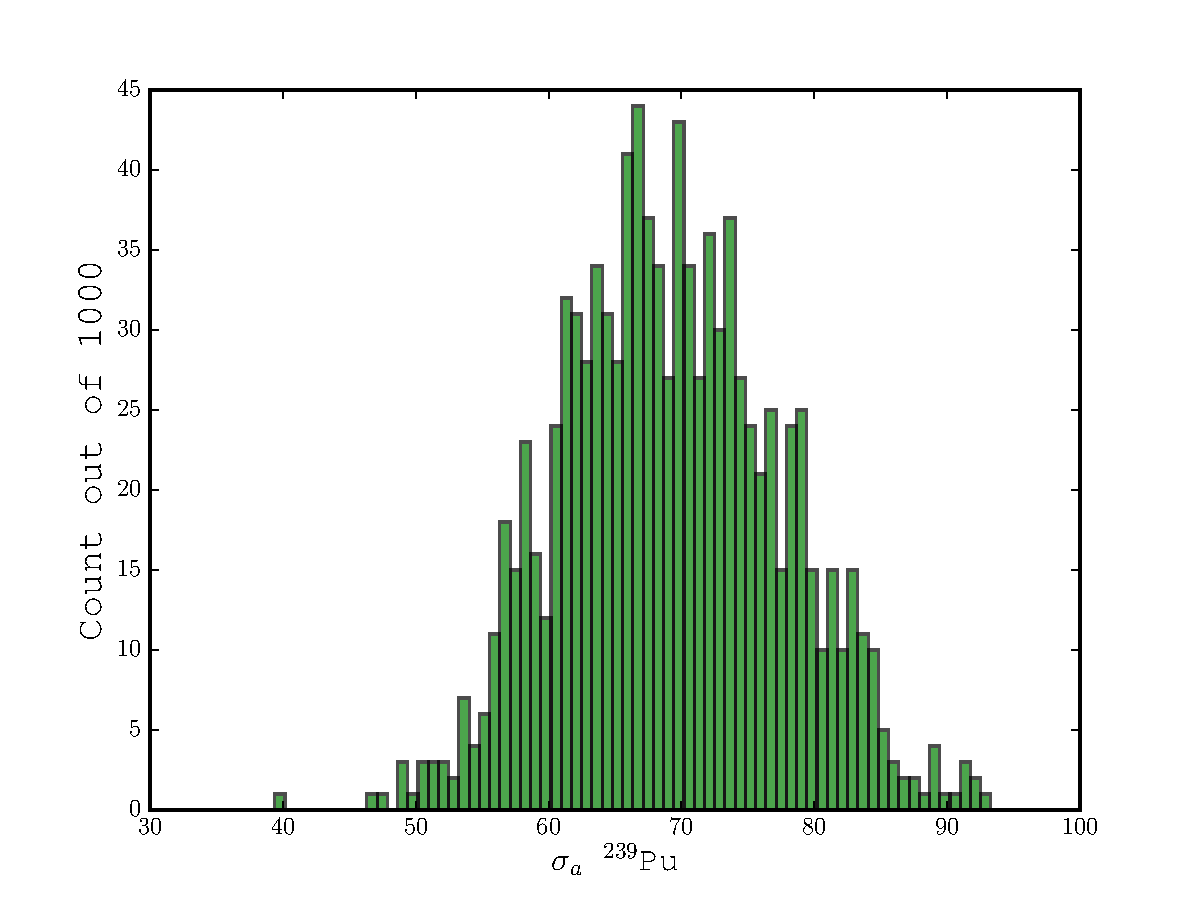
\includegraphics[width=1\columnwidth]{../Origen2/PLOTS/94Pu239aHIST.pdf}
      \vspace{-5mm}
      \label{fig:SPu239a}
    \end{center}
  \end{figure}
\end{frame}


\begin{frame}
  \begin{figure}[H]
    \begin{center}
      \hspace*{-0.6cm}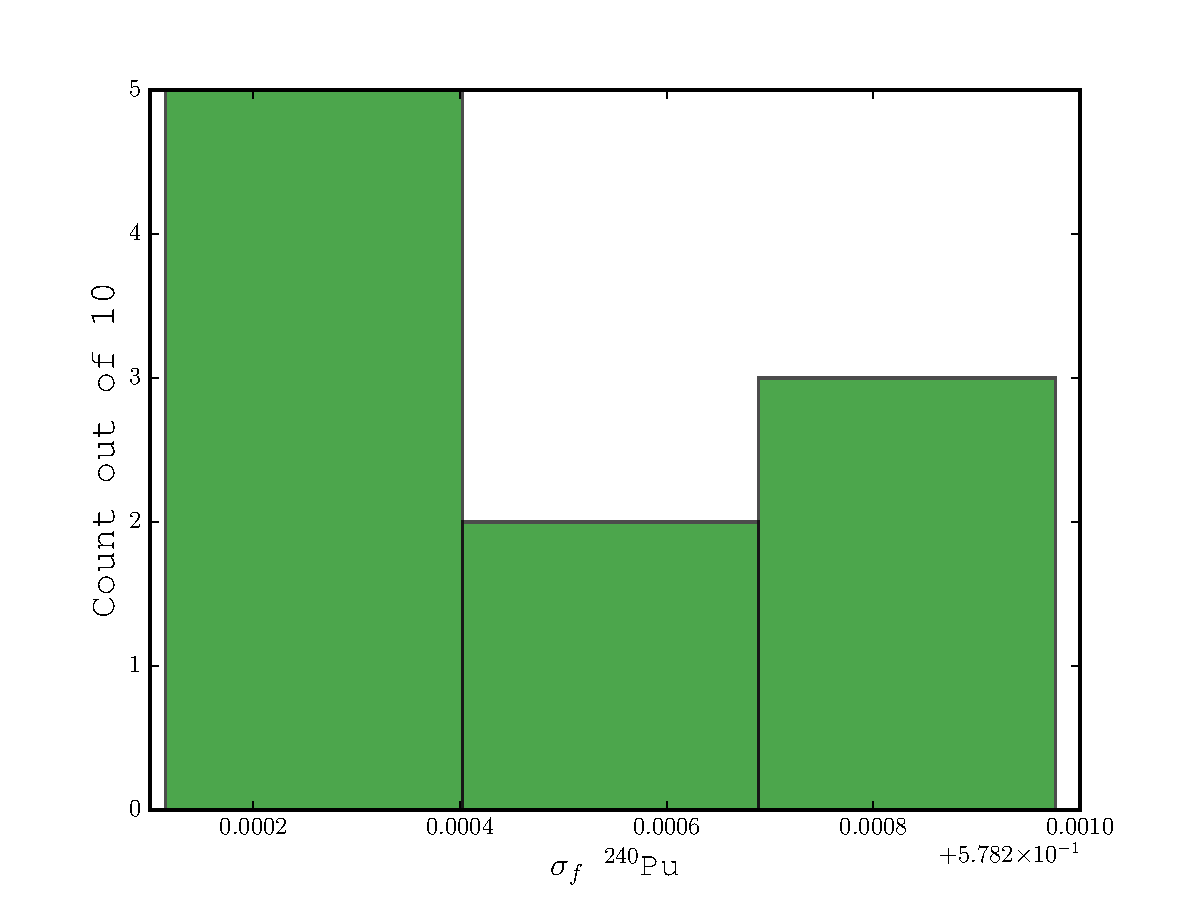
\includegraphics[width=1\columnwidth]{../Origen2/PLOTS/94Pu240fHIST.pdf}
      \vspace{-5mm}
      \label{fig:SPu240f}
    \end{center}
  \end{figure}
\end{frame}


\begin{frame}
  \begin{block}{Objectives}
  \vspace{0.3cm}
  \begin{itemize}
  \item[\done]{Build ORIGEN2 model for thermal system, calculating
  concentrations of QOIs}
  \item[\wontfix]{Determine how to vary cross section inputs for calculation}
  \item[\done]{Determine variance of cross-sections}
  \item[\done]{Create a sampling space for all possible variations of
    calculations}
  \item[\done]{Write program to plot results}
  \end{itemize}
  \vspace{0.3cm}
\end{block}
\end{frame}

\section{Results}
\begin{frame}
\sectionpage
\end{frame}

\begin{frame}
  \begin{figure}[H]
    \begin{center}
      \hspace*{-0.6cm}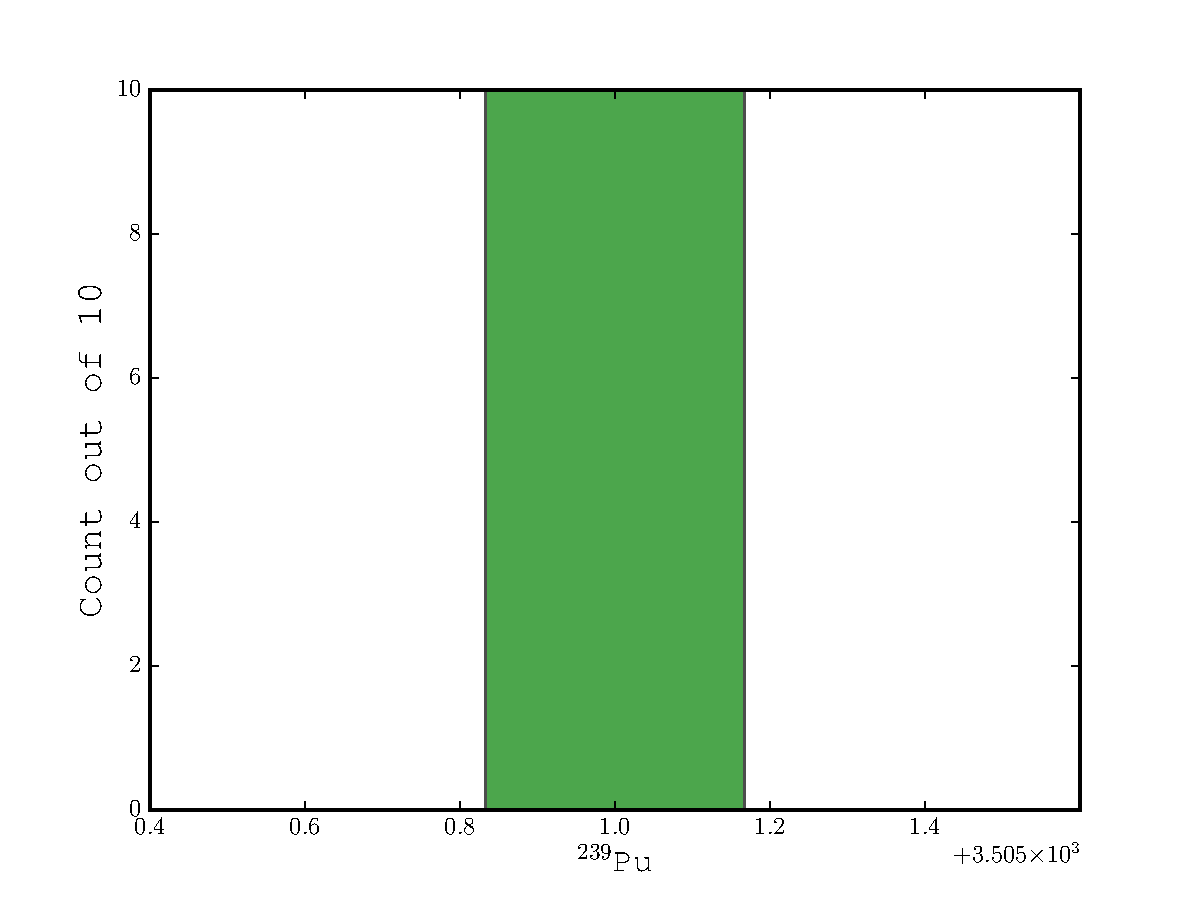
\includegraphics[width=1\columnwidth]{../Origen2/PLOTS/PU239Post_HIST.pdf}
      \vspace{-5mm}
      \label{fig:POSTHISTPu239}
    \end{center}
  \end{figure}
\end{frame}

\begin{frame}
    \begin{figure}[H]
    \begin{center}
      \hspace*{-0.6cm}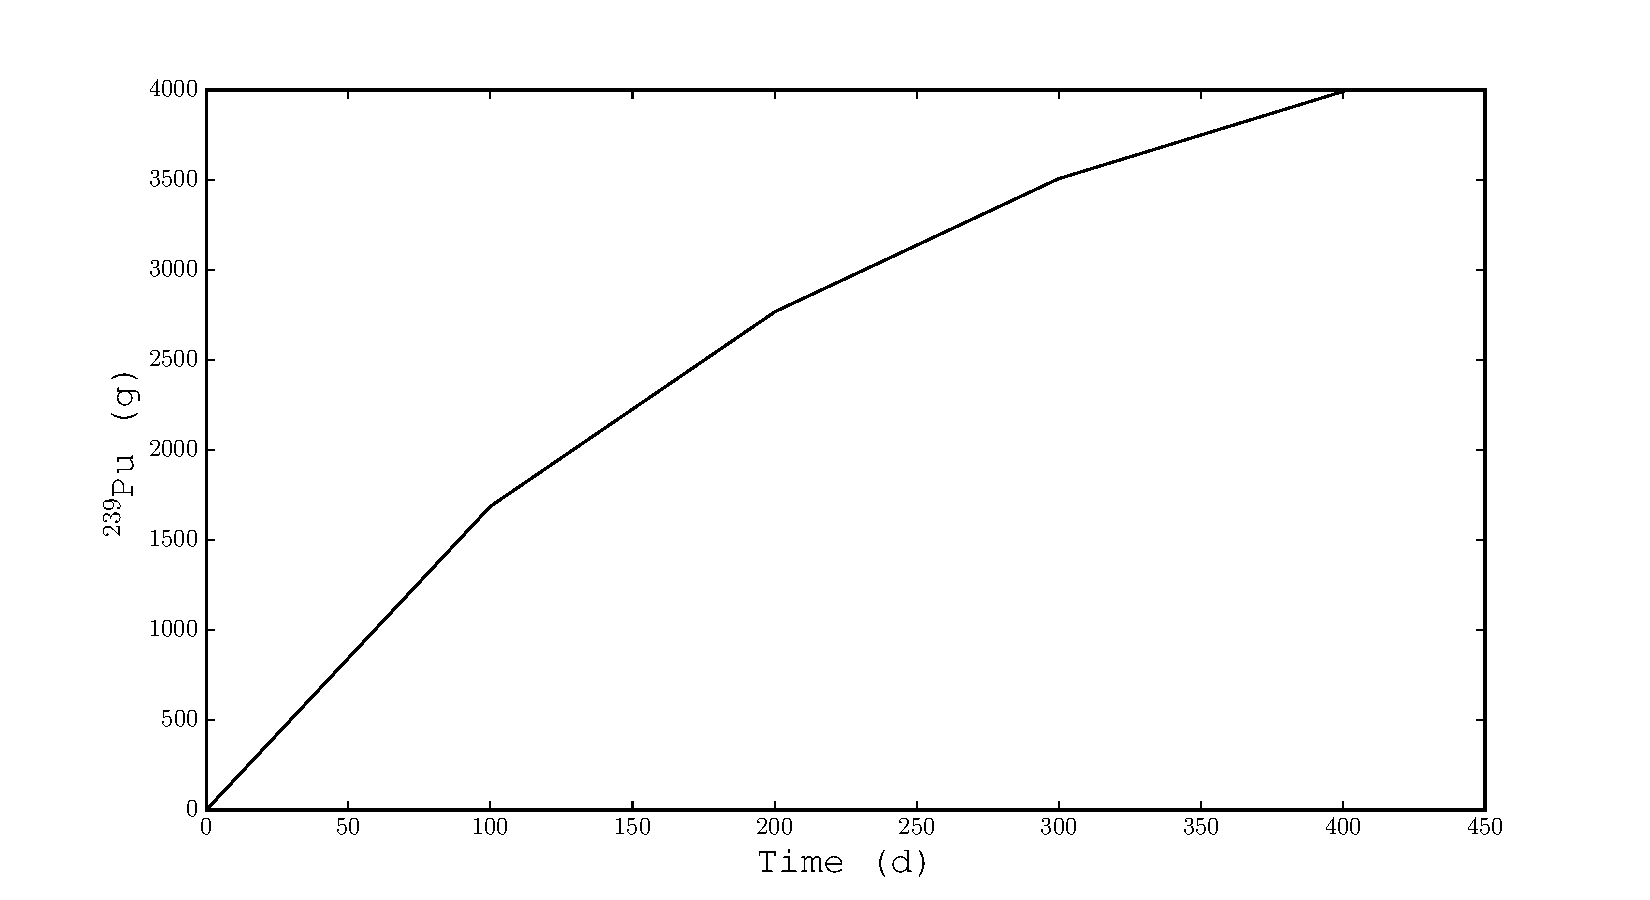
\includegraphics[width=1.1\columnwidth]{../Origen2/PLOTS/PU239Post_XY.pdf}
      \vspace{-5mm}
    \end{center}
  \end{figure}
\end{frame}


\begin{frame}
  \begin{figure}[H]
    \begin{center}
      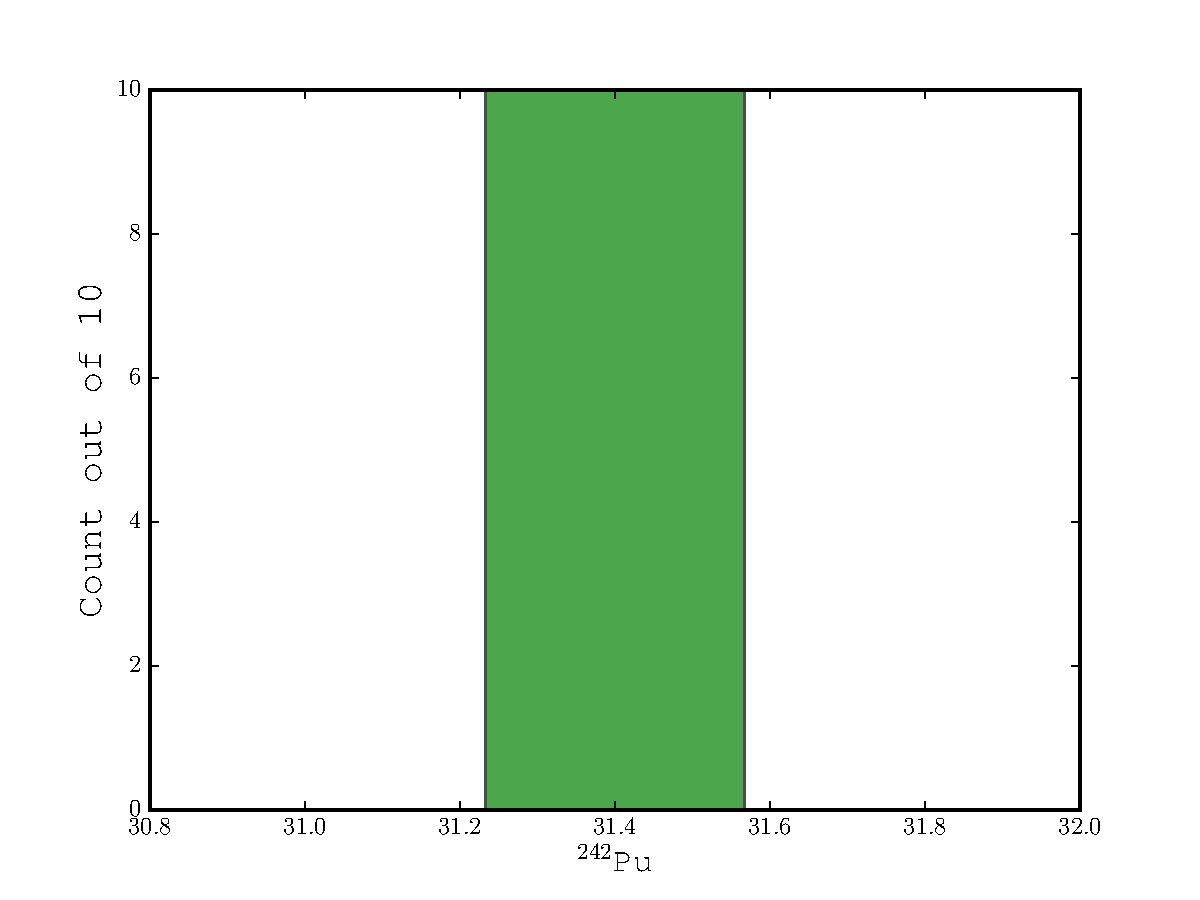
\includegraphics[width=0.77\columnwidth]{../Origen2/PLOTS/PU242Post_HIST.pdf}
      \vspace{-5mm}
      \label{fig:POSTHISTPu242}
    \end{center}
  \end{figure}
\end{frame}
  
\begin{frame}
    \begin{figure}[H]
    \begin{center}
      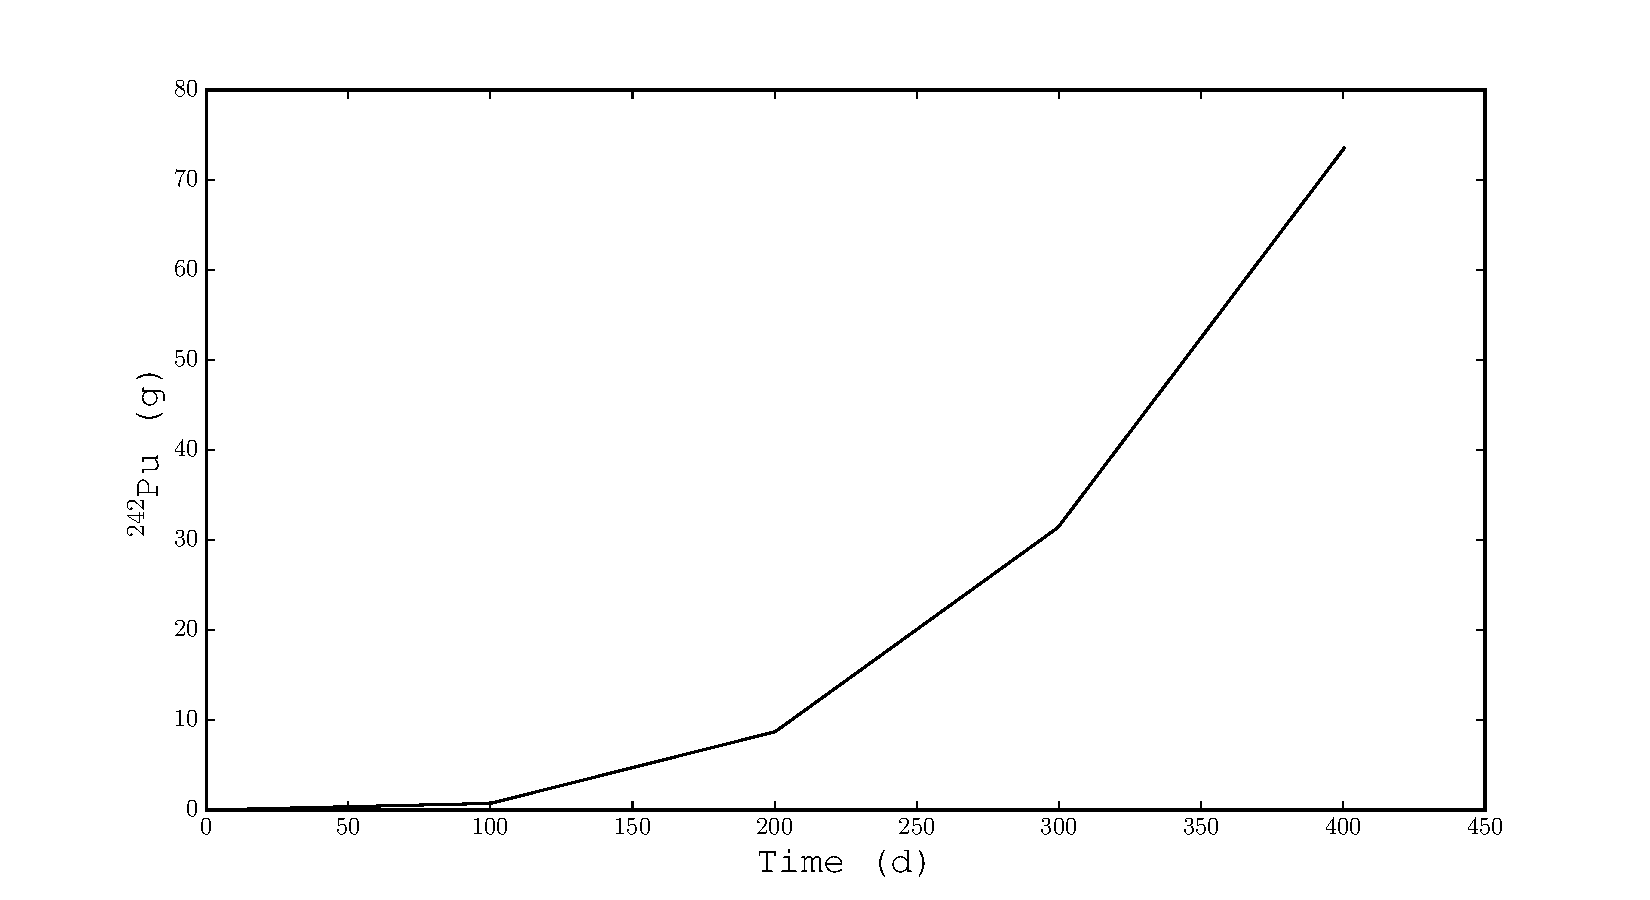
\includegraphics[width=0.77\columnwidth]{../Origen2/PLOTS/PU242Post_XY.pdf}
      \vspace{-5mm}
      \label{fig:POSTXYPu242}
    \end{center}
  \end{figure}
\end{frame}
    
\begin{frame}
  \begin{figure}[H]
    \begin{center}
      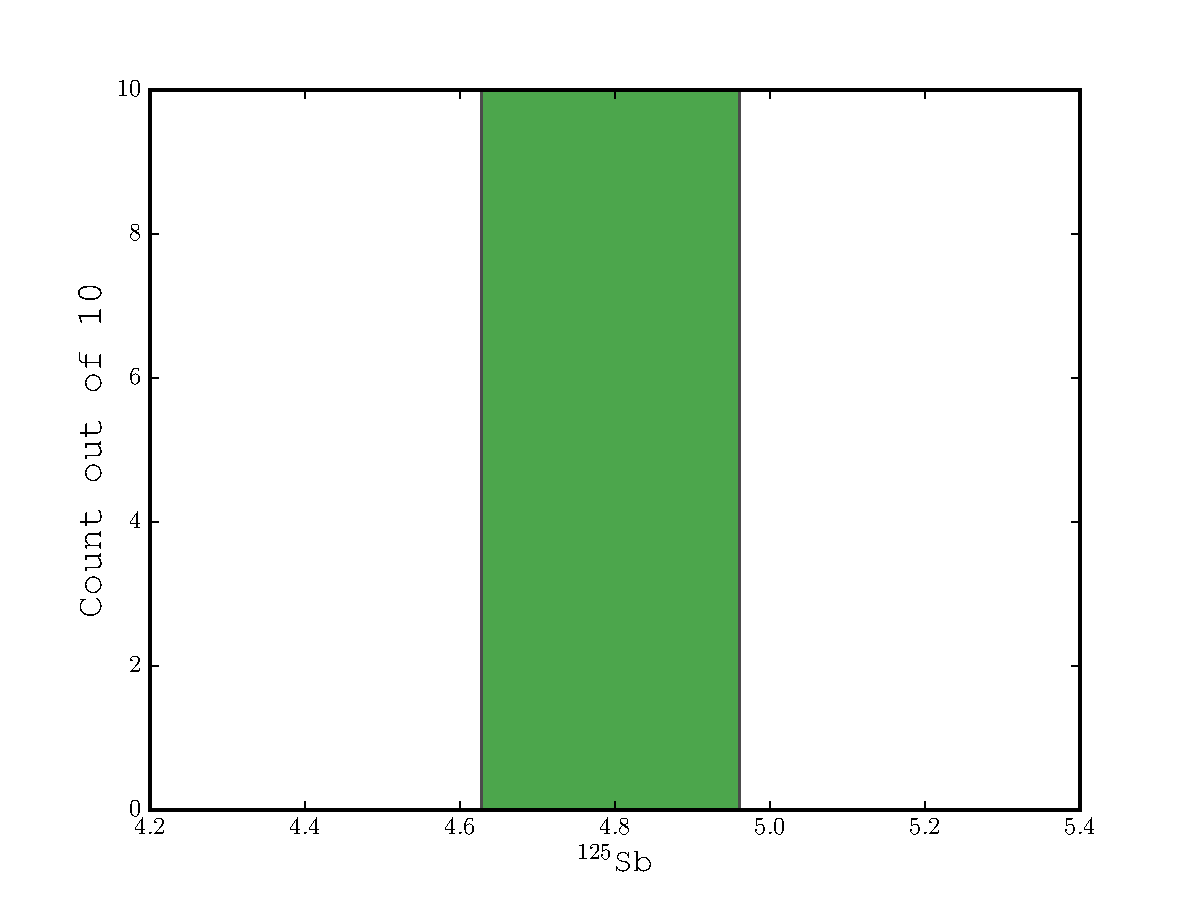
\includegraphics[width=0.77\columnwidth]{../Origen2/PLOTS/SB125Post_HIST.pdf}
      \vspace{-5mm}
      \label{fig:POSTHISTSb125}
    \end{center}
  \end{figure}
\end{frame}
  
\begin{frame}
    \begin{figure}[H]
    \begin{center}
      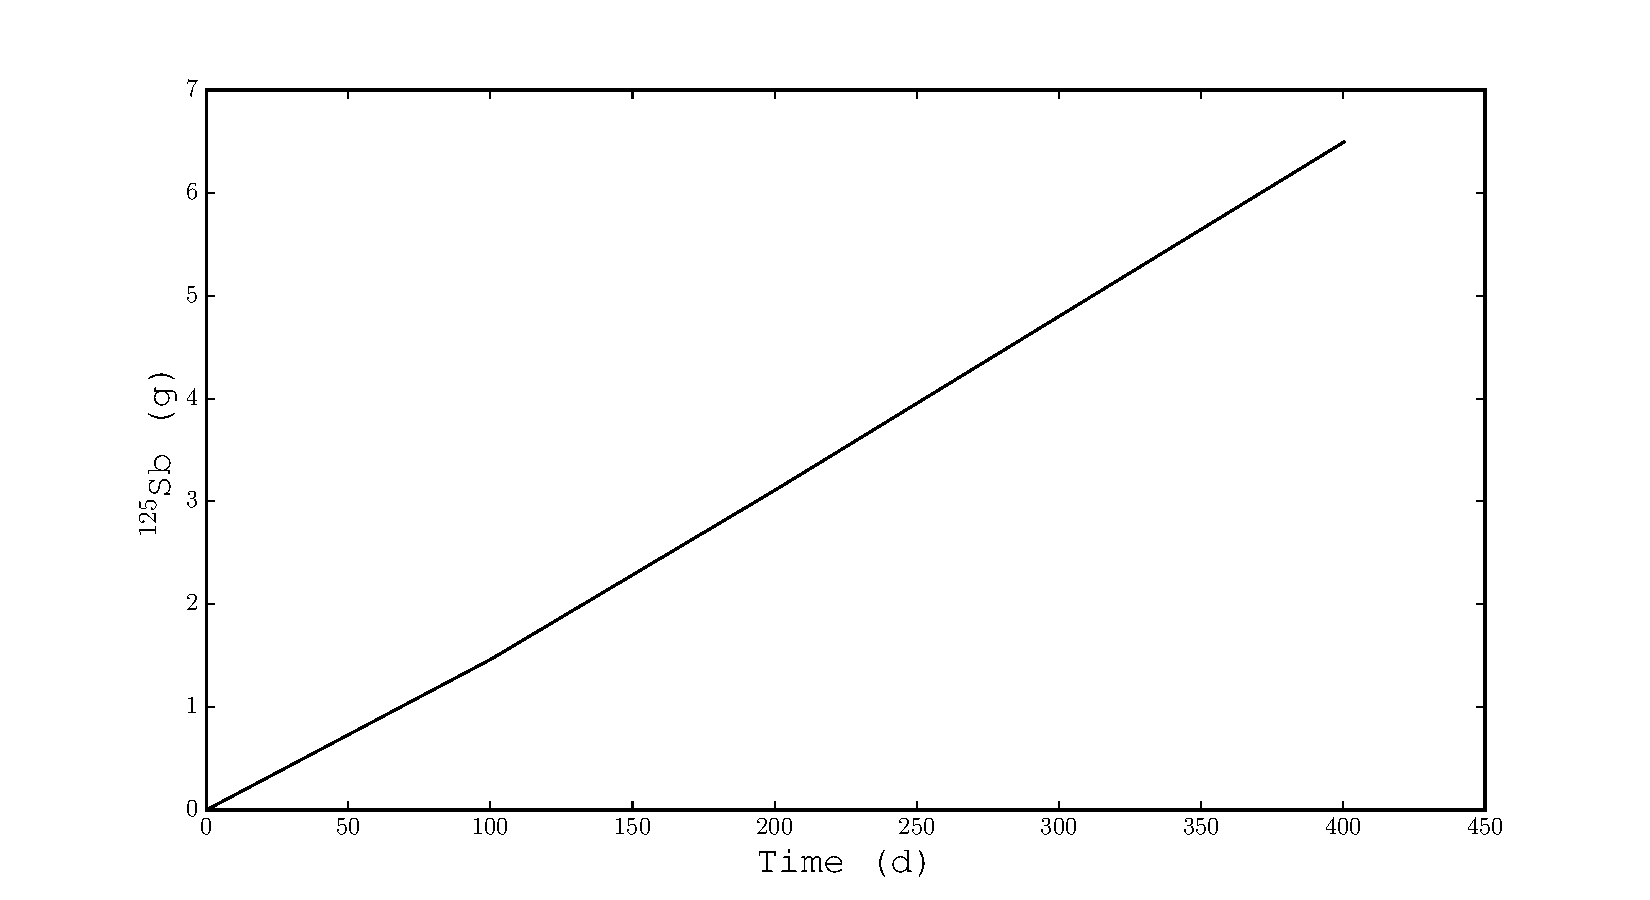
\includegraphics[width=0.77\columnwidth]{../Origen2/PLOTS/SB125Post_XY.pdf}
      \vspace{-5mm}
      \label{fig:POSTXYSb125}
    \end{center}
  \end{figure}
\end{frame}
    
\begin{frame}
  \begin{figure}[H]
    \begin{center}
      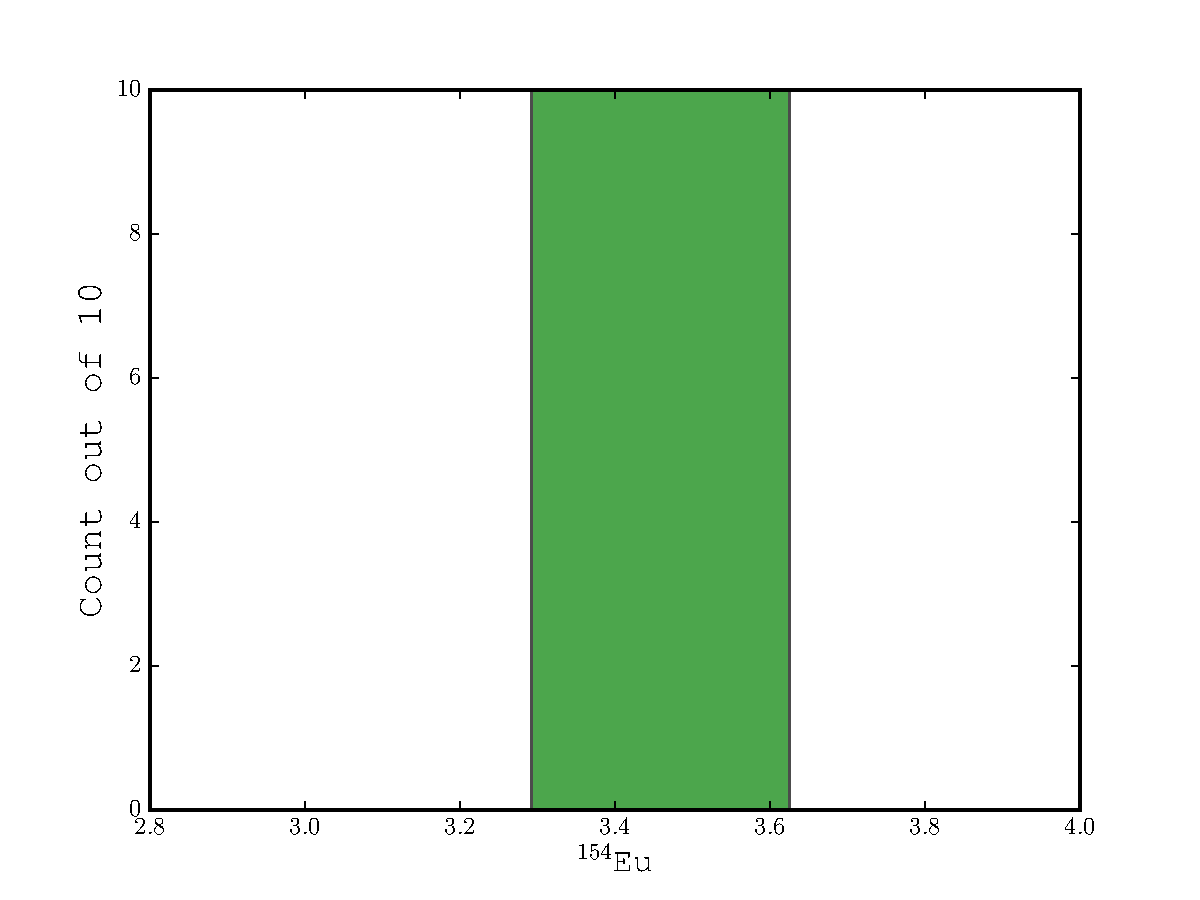
\includegraphics[width=0.77\columnwidth]{../Origen2/PLOTS/EU154Post_HIST.pdf}
      \vspace{-5mm}
      \label{fig:POSTHISTEu154}
    \end{center}
  \end{figure}
\end{frame}
  
\begin{frame}
    \begin{figure}[H]
    \begin{center}
      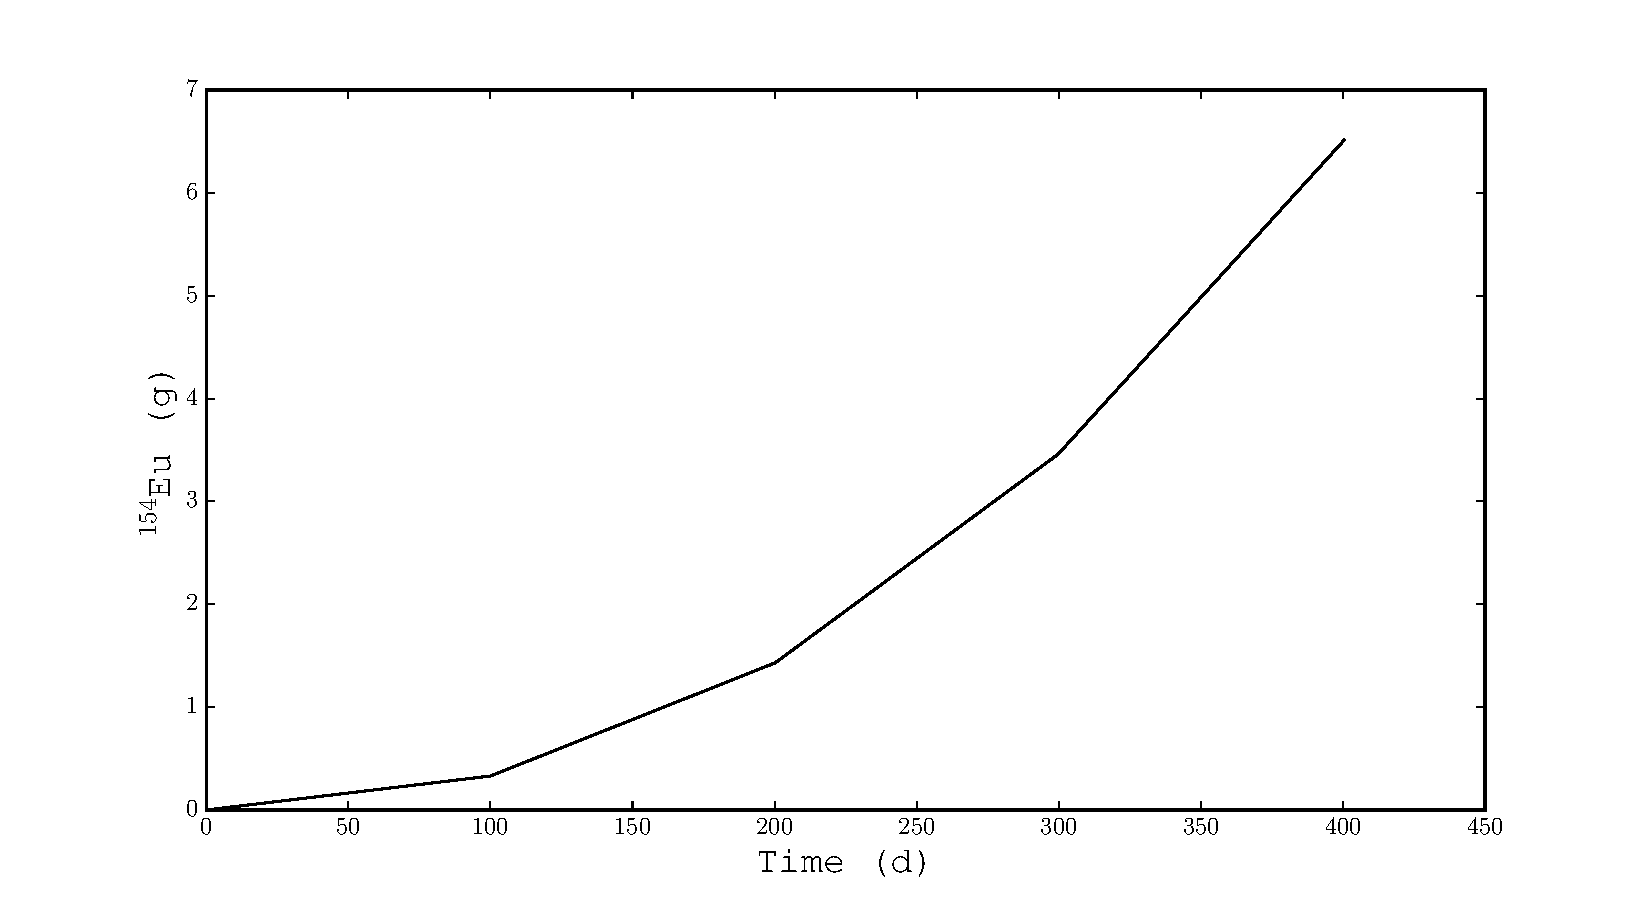
\includegraphics[width=0.77\columnwidth]{../Origen2/PLOTS/EU154Post_XY.pdf}
      \vspace{-5mm}
      \label{fig:POSTXYEu154}
    \end{center}
  \end{figure}
\end{frame}
    
\begin{frame}
  \begin{figure}[H]
    \begin{center}
      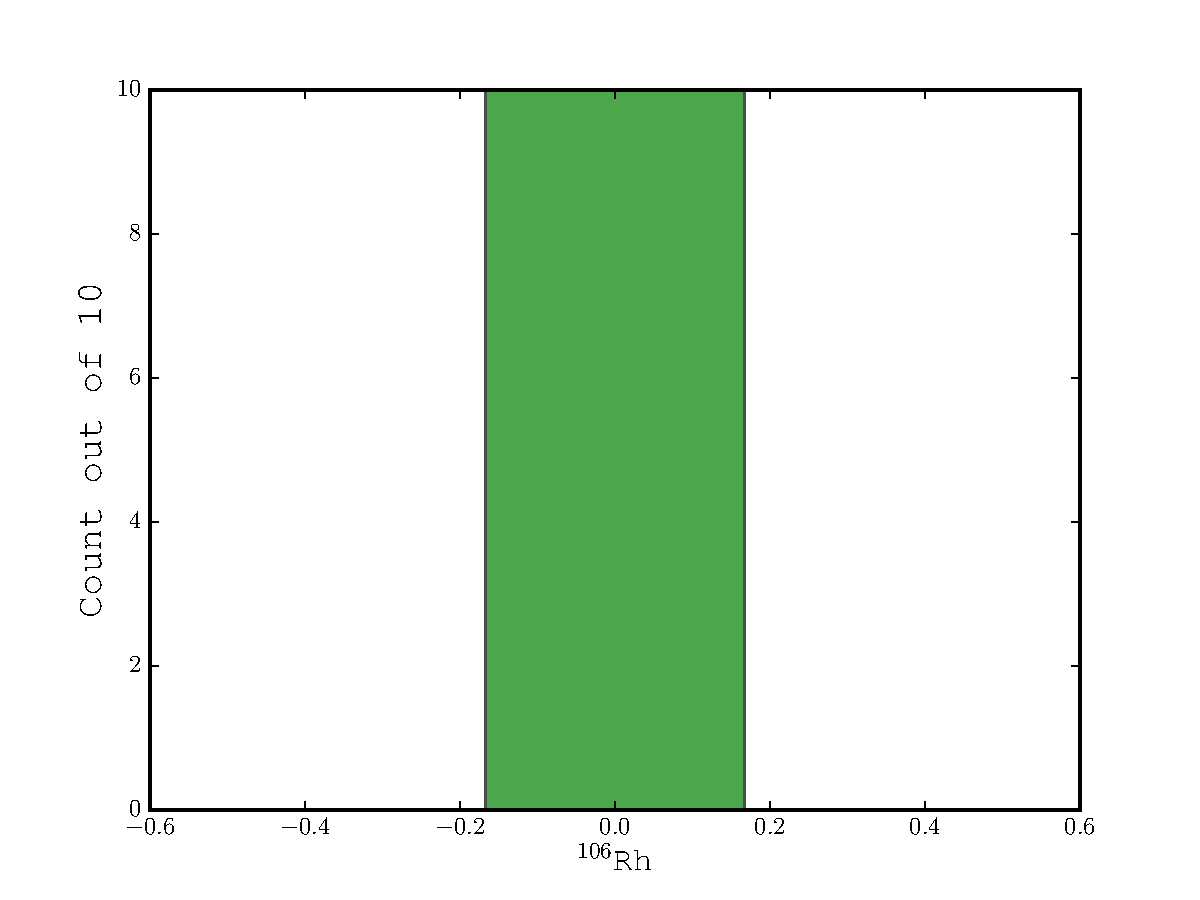
\includegraphics[width=0.77\columnwidth]{../Origen2/PLOTS/RH106Post_HIST.pdf}
      \vspace{-5mm}
      \label{fig:POSTHISTRh106}
    \end{center}
  \end{figure}
\end{frame}
  
\begin{frame}
    \begin{figure}[H]
    \begin{center}
      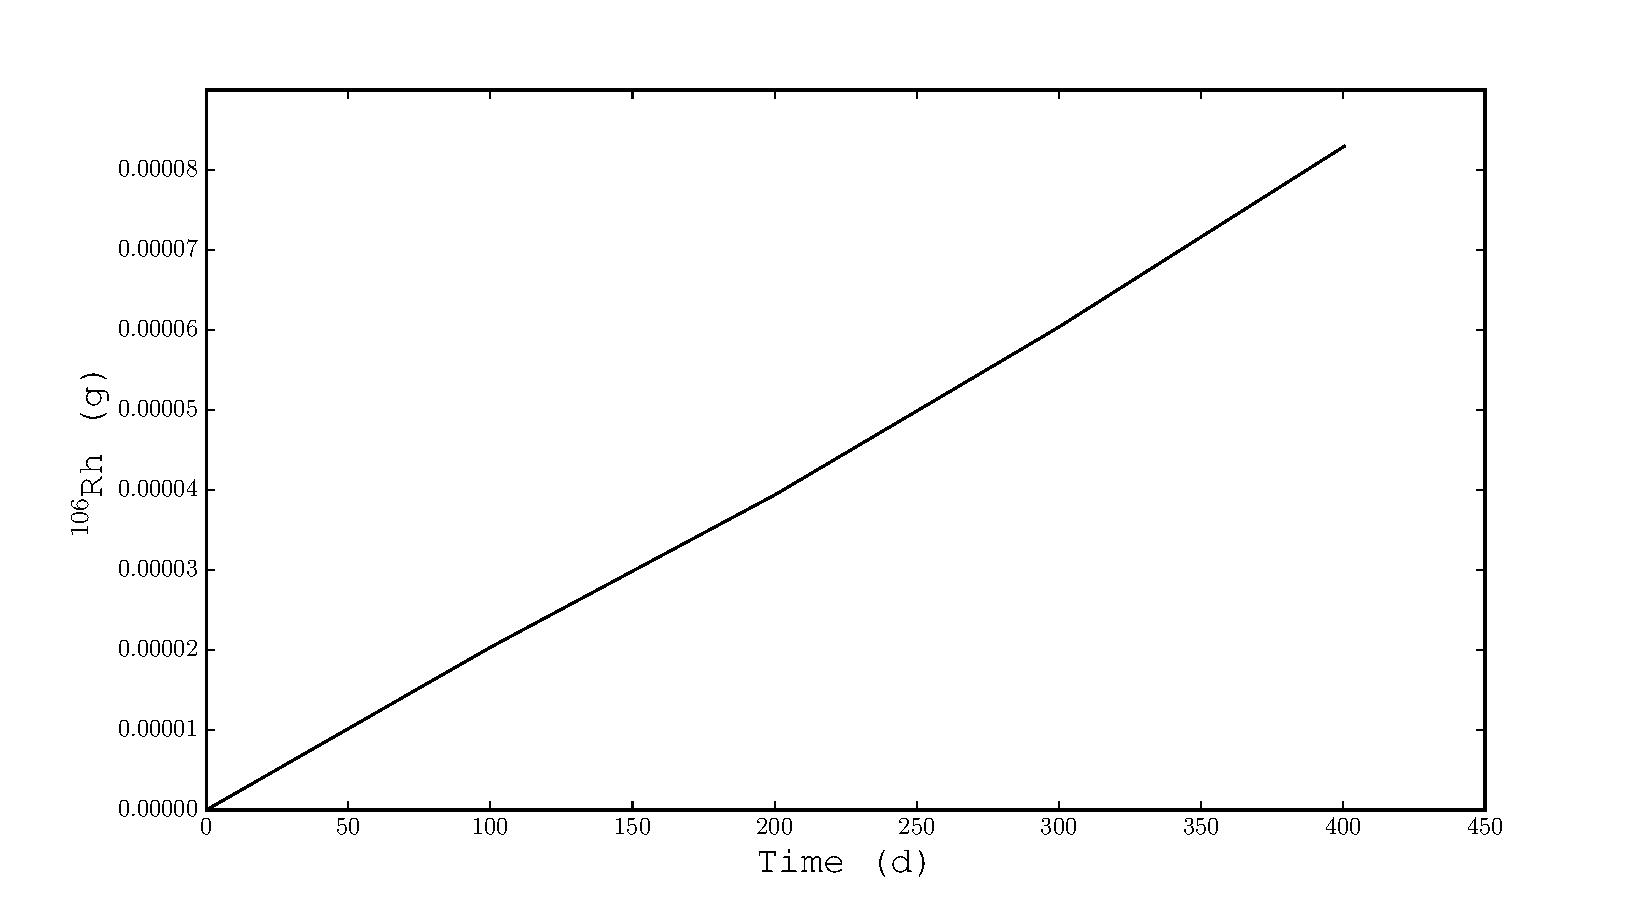
\includegraphics[width=0.77\columnwidth]{../Origen2/PLOTS/RH106Post_XY.pdf}
      \vspace{-5mm}
      \label{fig:POSTXYRh106}
    \end{center}
  \end{figure}
\end{frame}
    
\begin{frame}
  \begin{figure}[H]
    \begin{center}
      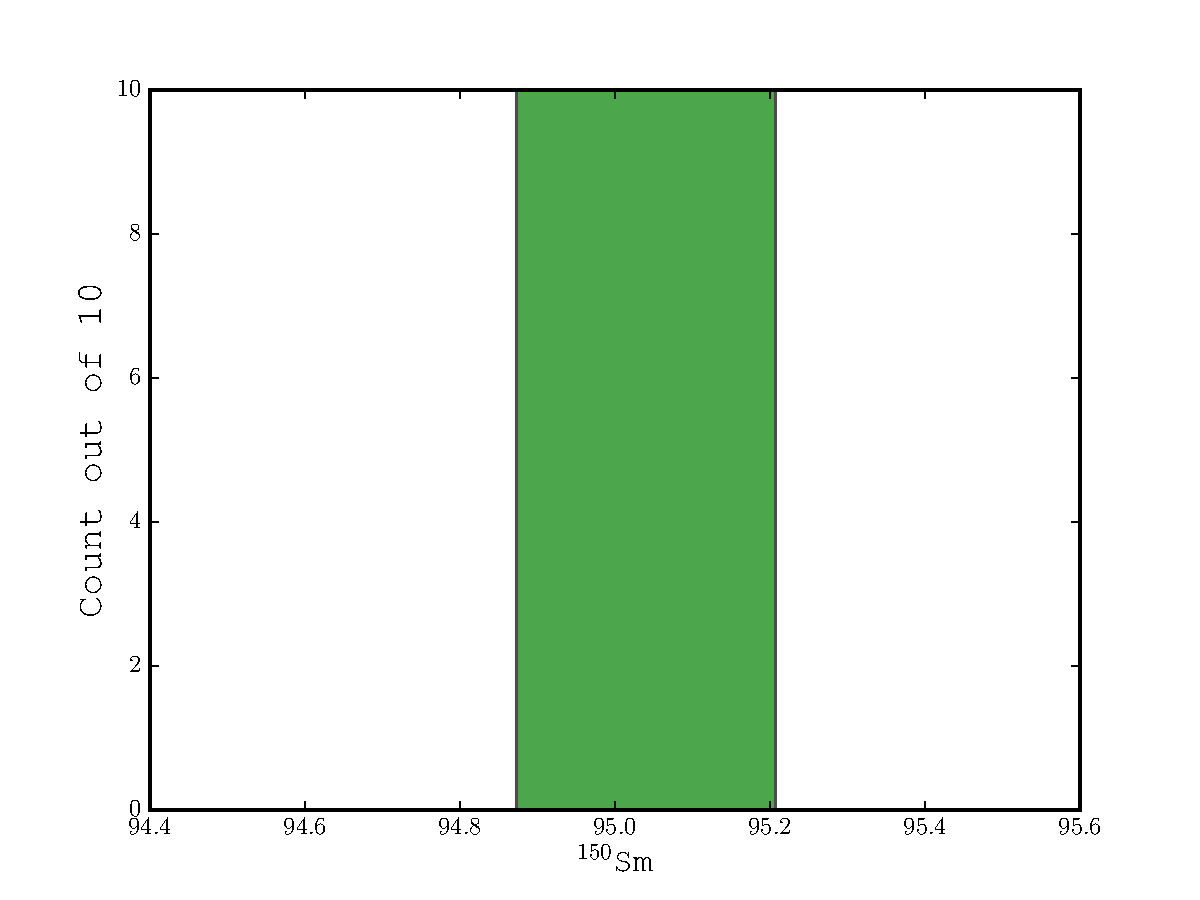
\includegraphics[width=0.77\columnwidth]{../Origen2/PLOTS/SM150Post_HIST.pdf}
      \vspace{-5mm}
      \label{fig:POSTHISTSm150}
    \end{center}
  \end{figure}
\end{frame}
  
\begin{frame}
    \begin{figure}[H]
    \begin{center}
      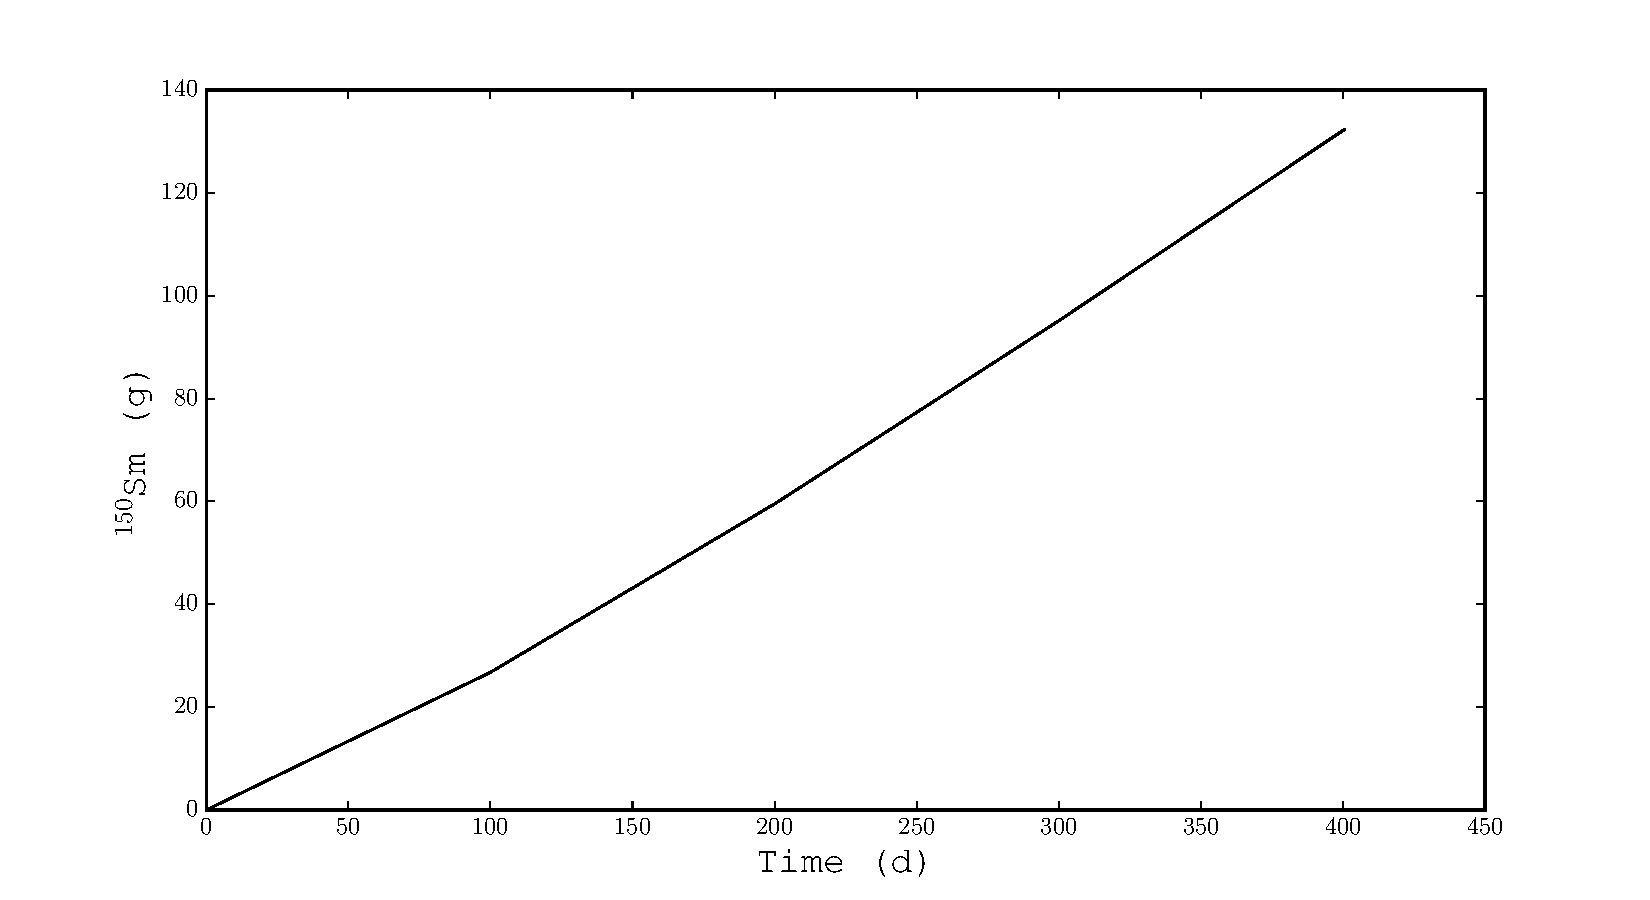
\includegraphics[width=0.77\columnwidth]{../Origen2/PLOTS/SM150Post_XY.pdf}
      \vspace{-5mm}
      \label{fig:POSTXYSm150}
    \end{center}
  \end{figure}
\end{frame}
    
\begin{frame}
  \begin{figure}[H]
    \begin{center}
      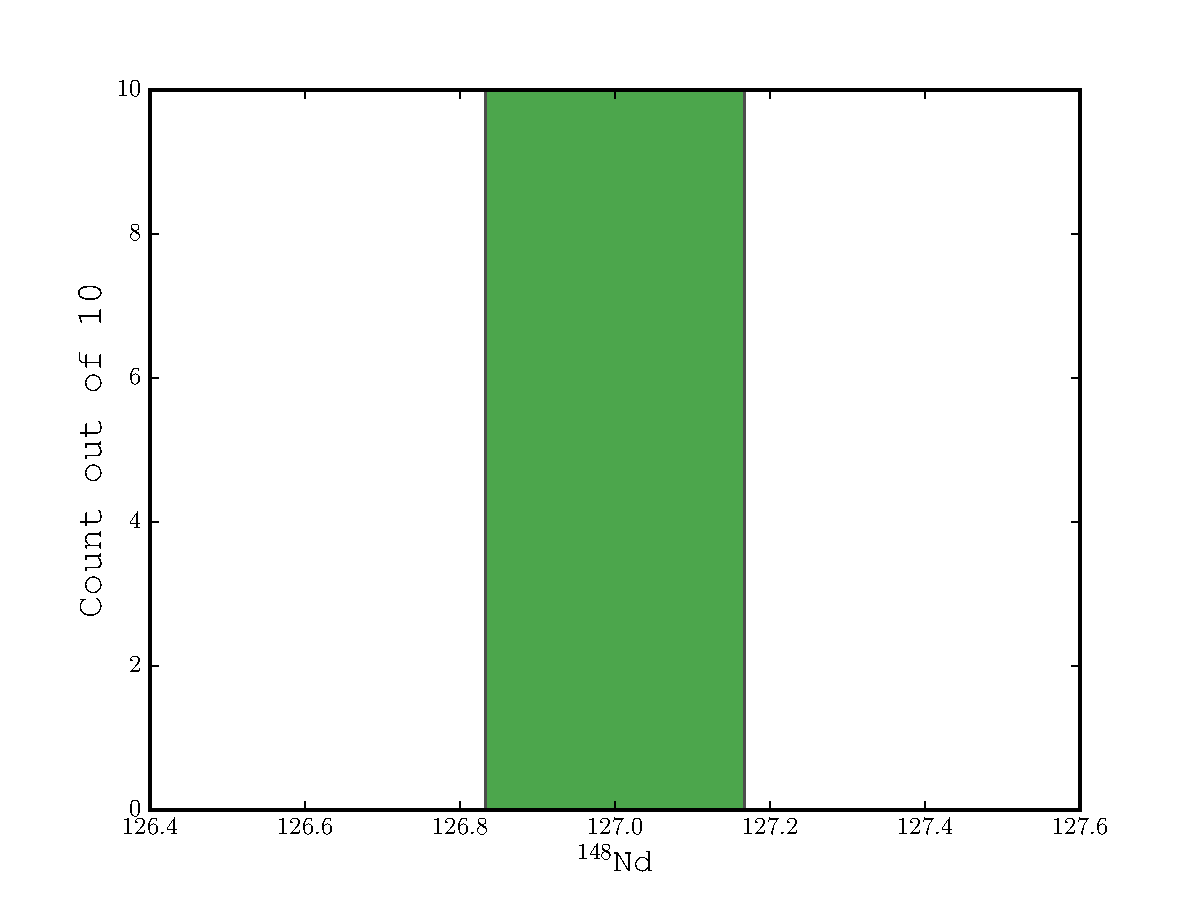
\includegraphics[width=0.77\columnwidth]{../Origen2/PLOTS/ND148Post_HIST.pdf}
      \vspace{-5mm}
      \label{fig:POSTHISTNd148}
    \end{center}
  \end{figure}
\end{frame}
  
\begin{frame}
    \begin{figure}[H]
    \begin{center}
      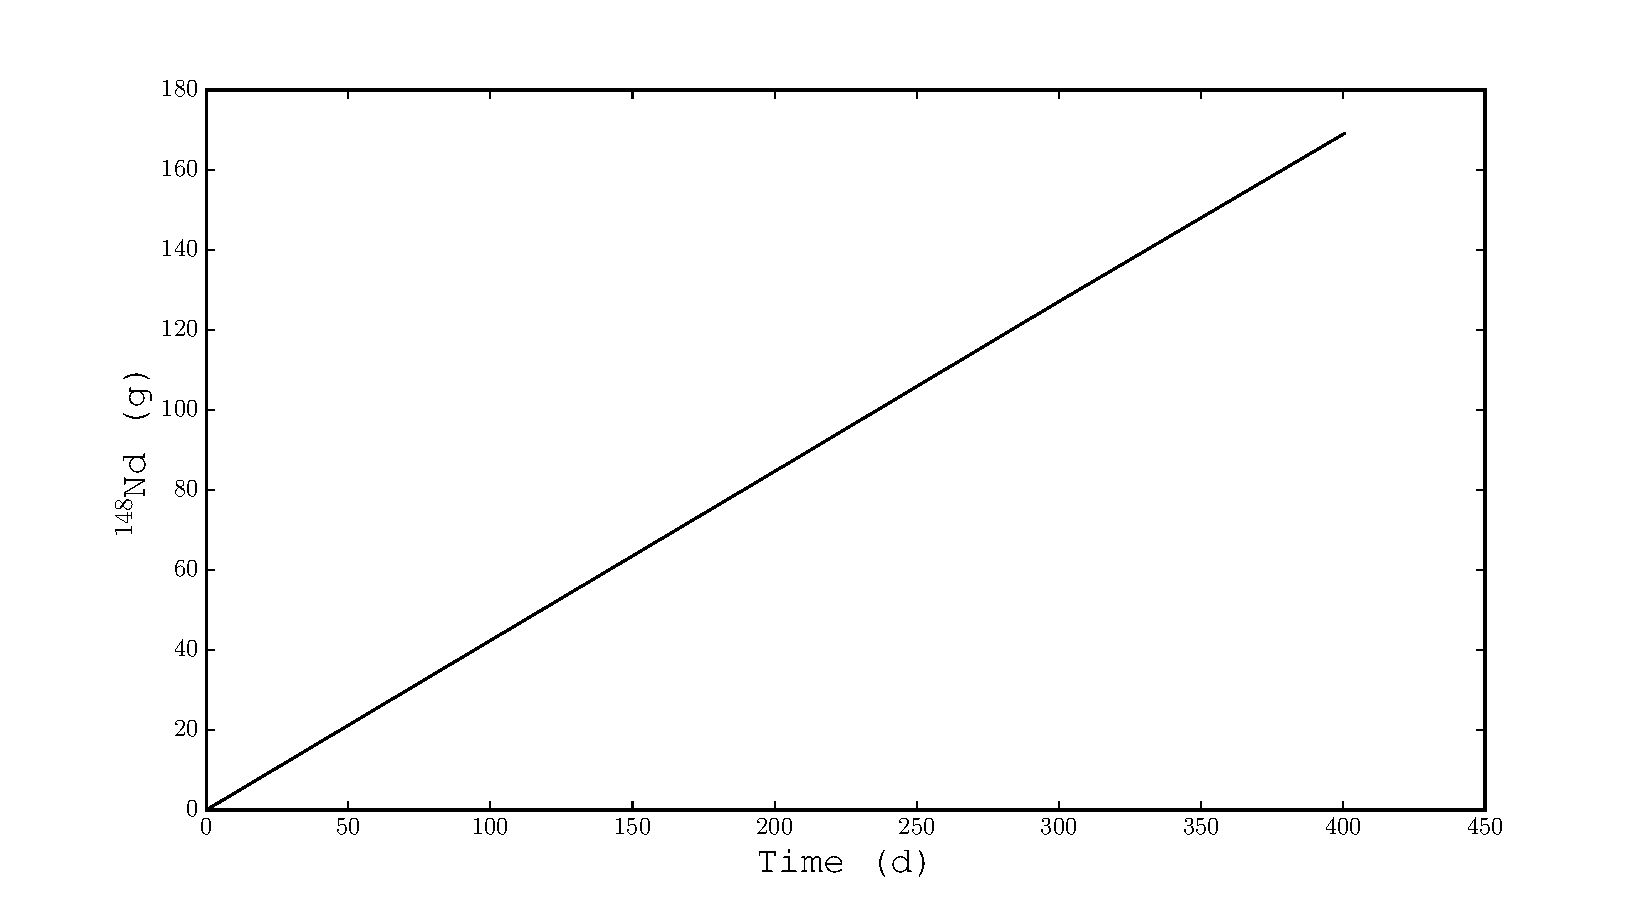
\includegraphics[width=0.77\columnwidth]{../Origen2/PLOTS/ND148Post_XY.pdf}
      \vspace{-5mm}
      \label{fig:POSTXYNd148}
    \end{center}
  \end{figure}
\end{frame}
    
\begin{frame}
  \begin{figure}[H]
    \begin{center}
      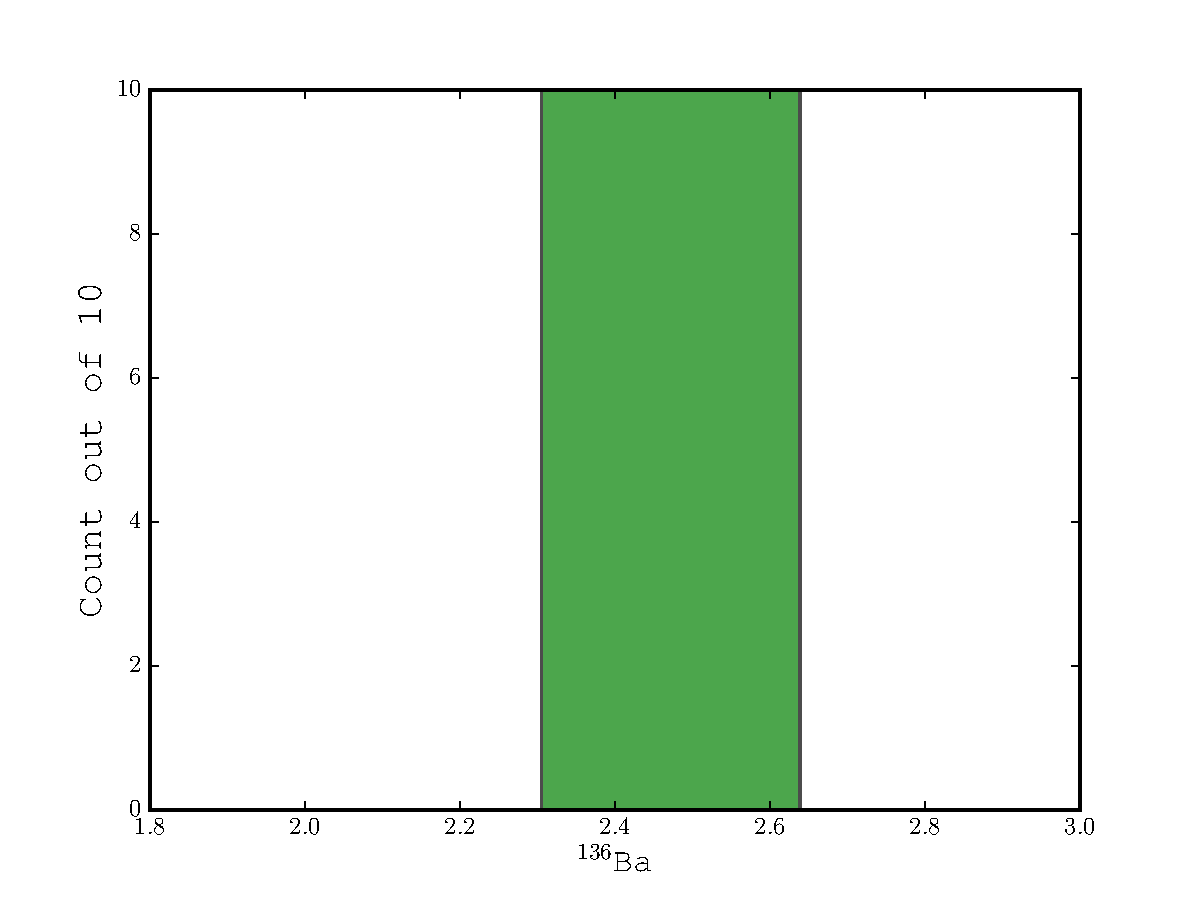
\includegraphics[width=0.77\columnwidth]{../Origen2/PLOTS/BA136Post_HIST.pdf}
      \vspace{-5mm}
      \label{fig:POSTHISTBa136}
    \end{center}
  \end{figure}
\end{frame}
  
\begin{frame}
    \begin{figure}[H]
    \begin{center}
      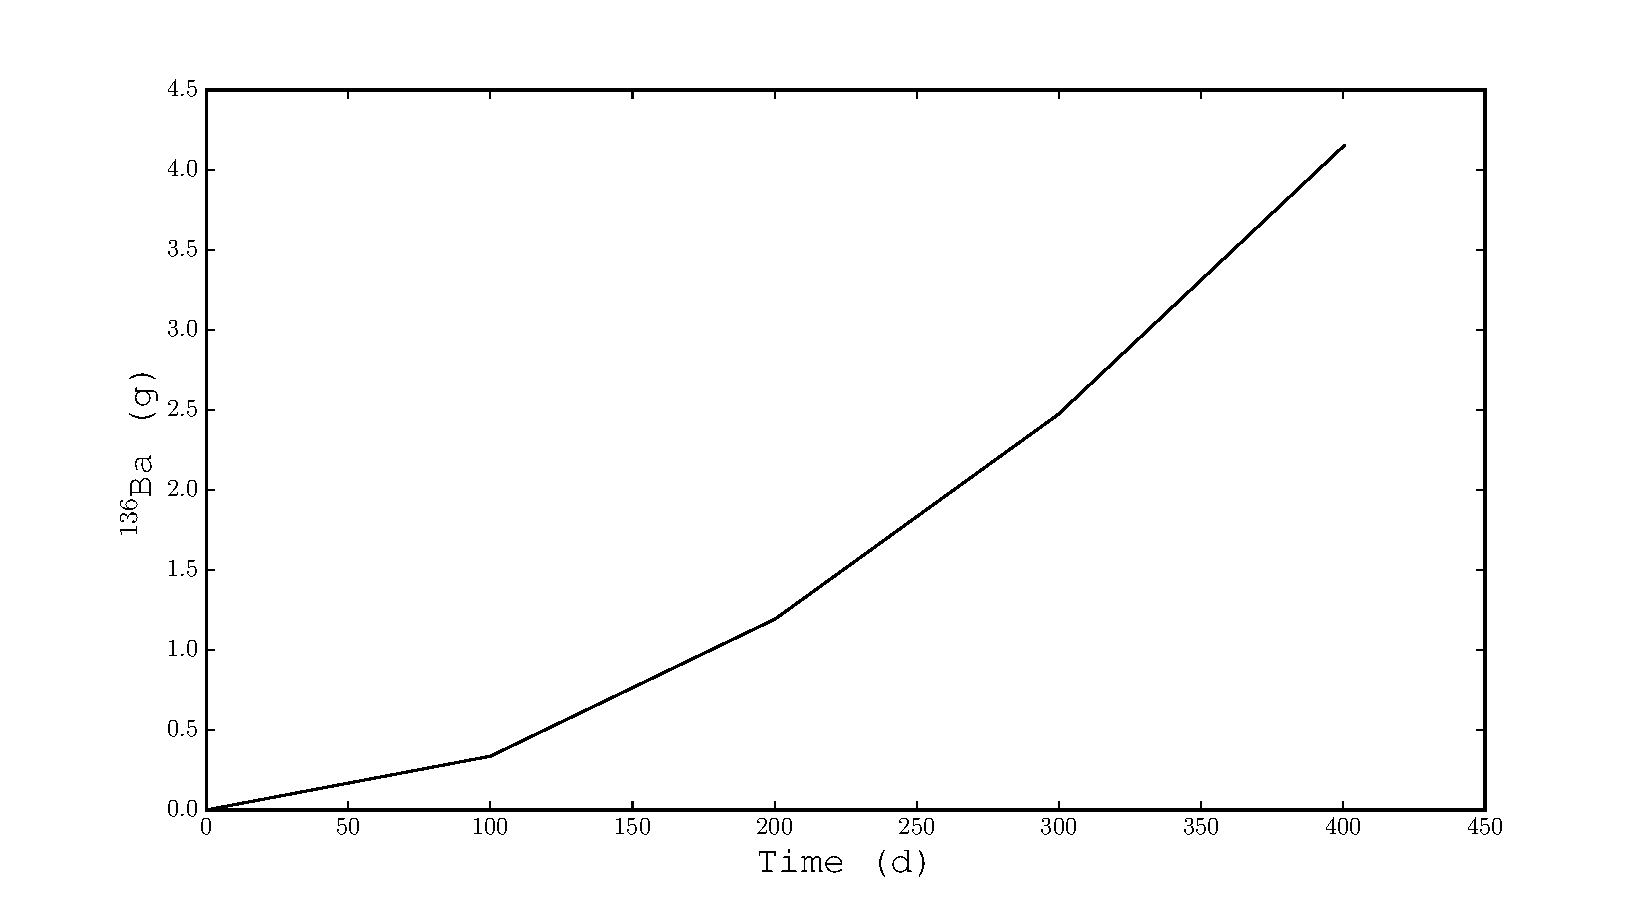
\includegraphics[width=0.77\columnwidth]{../Origen2/PLOTS/BA136Post_XY.pdf}
      \vspace{-5mm}
      \label{fig:POSTXYBa136}
    \end{center}
  \end{figure}
\end{frame}
    
\begin{frame}
  \begin{figure}[H]
    \begin{center}
      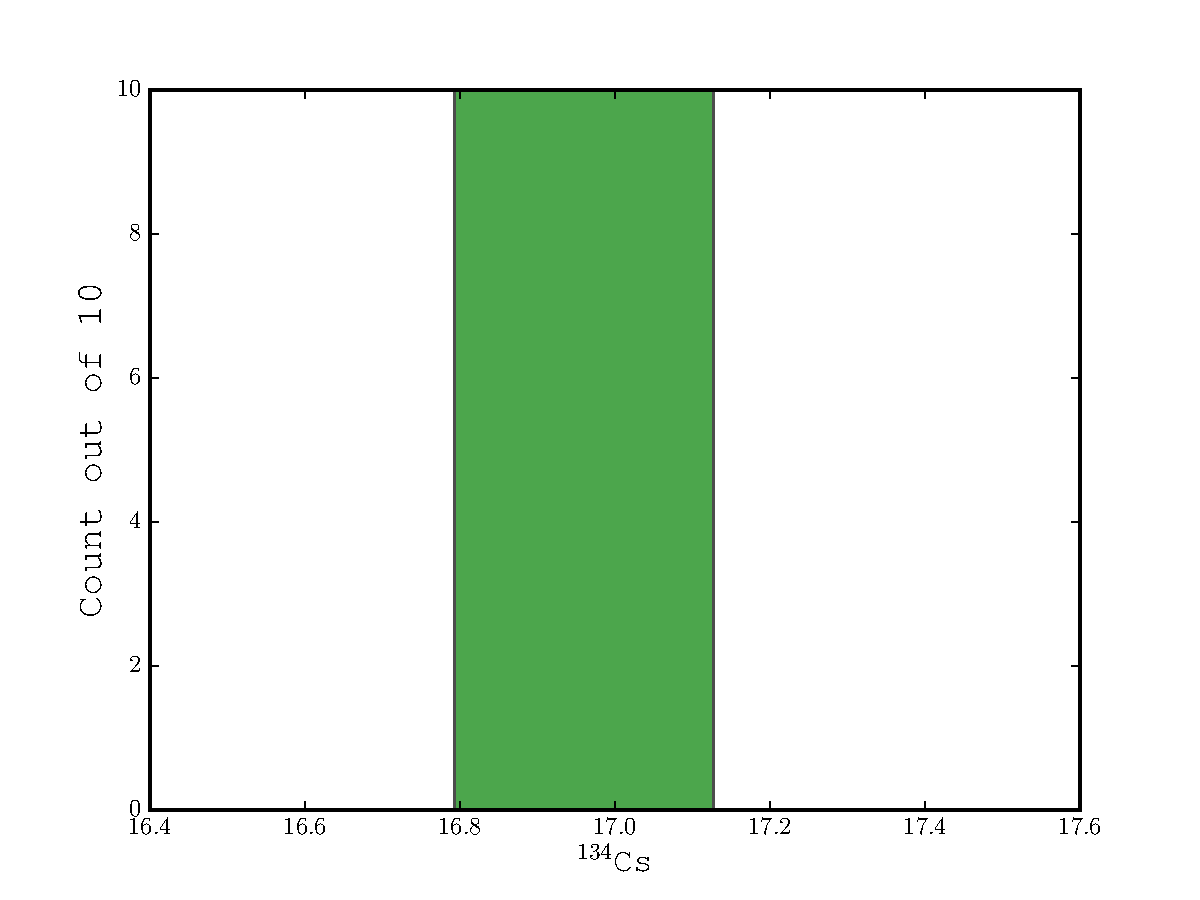
\includegraphics[width=0.77\columnwidth]{../Origen2/PLOTS/CS134Post_HIST.pdf}
      \vspace{-5mm}
      \label{fig:POSTHISTBa136}
    \end{center}
  \end{figure}
\end{frame}
  
\begin{frame}
    \begin{figure}[H]
    \begin{center}
      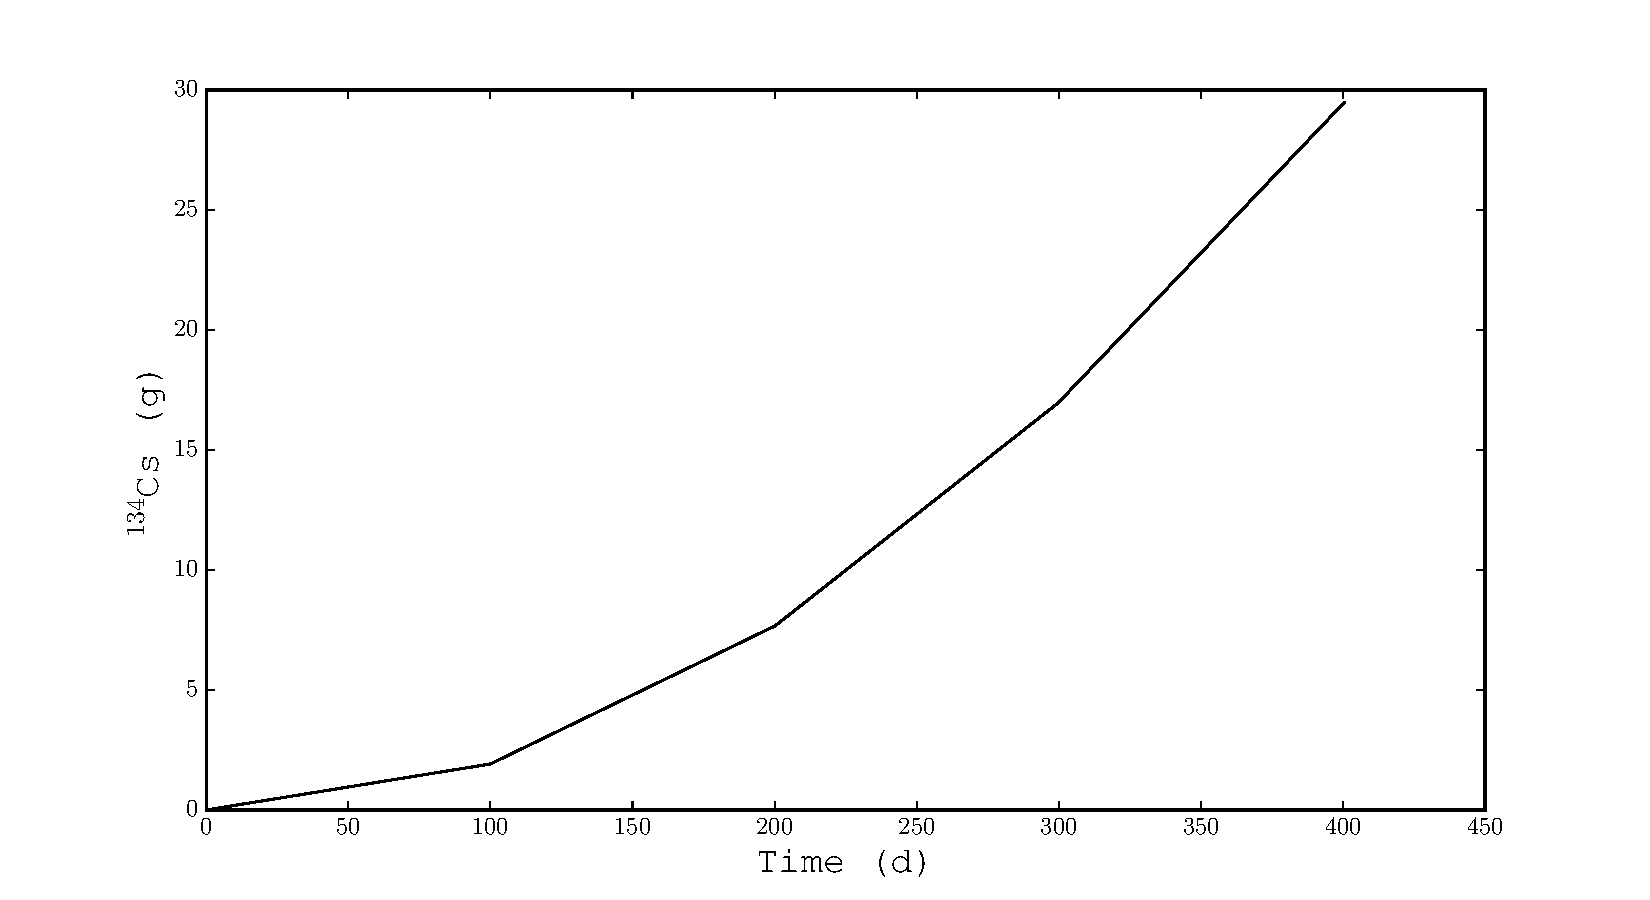
\includegraphics[width=0.77\columnwidth]{../Origen2/PLOTS/CS134Post_XY.pdf}
      \vspace{-5mm}
      \label{fig:POSTXYCs134}
    \end{center}
  \end{figure}
\end{frame}


\section{Conclusions}
\begin{frame}{Conclusions}
  \begin{itemize}
  \item{Surprised at size of error}
  \item{Sad it didn't work fully}
  \end{itemize}
\end{frame}

\end{document}
